\newpage

%%%%%%%%%%%%%%%%%%%%%%%%%%%%%%%%%%%%%%%
%% NEW CHAPTER
%%%%%%%%%%%%%%%%%%%%%%%%%%%%%%%%%%%%%%%

\section{Populations}
{\it 
The previous chapter developed a model of individual behaviour based on an
assumed dynamic imposed on wealth. If we know the stochastic process that describes
individual wealth, then we also know what happens at population level -- each individual
is represented by a realisation of the process, and we can compute 
the dynamics of wealth distributions. We answer questions about inequality and poverty in
a model economy which, for the moment, contains no interactions between individuals. We also gain an understanding of when and how results for finite populations differ from those for the infinite ensemble.}
\newpage

%%%%%%%%%%%%%%%%%%%%%%%%%%%%%%%%%%%%%%%

\subsection{Every man for himself}
\seclabel{Every_man}

We have seen that risk aversion constitutes optimal behaviour under the assumption 
of multiplicative wealth growth and over time scales that are long enough for systematic 
trends to be significant. In this chapter we will continue to explore our null model, 
\GBM. By ``explore'' we mean that we will let the model generate its world -- if 
individual wealth was to follow \GBM, what kind of features of an economy would emerge? 
We will see that cooperation and the formation of social structure also constitute 
optimal behaviour.

\GBM is more than a random variable. It's a stochastic process, either a set of trajectories 
or a family of time-dependent random variables, depending on how we 
prefer to look at it.  Both perspectives are informative in the context of economic modelling:
from the set of trajectories we can judge what is likely to happen to an individual, 
\eg by following a single trajectory for a long time; while the \PDFa of the random 
variable $\x(\t^*)$ at some fixed value of $\t^*$ tells us how wealth is distributed in our model. 

We use the term wealth distribution to refer to the density function, $\PDF_\x(\x)$, and not the process of distributing wealth among people. This can be interpreted as follows. Imagine a population of $\N$ individuals. If I select a random individual, each having uniform probability $\frac{1}{\N}$, then the probability of the selected individual having wealth greater than $\x$ is given by the CDF, $F_\x(\x)=\int_\x^\infty \PDF_\x(s)\gd s$. If $\N$ is large, then $\D \x \PDF_\x(\x)\N$ is the approximate number of individuals who have wealth between $\x$ and $\x+\D \x$. Thus, a broad wealth distribution with heavy tails indicates greater wealth inequality.

\underline{Examples:}
\begin{itemize}
\item Under perfect equality everyone would have the same, meaning that the wealth
distribution would be a Dirac delta function centred at the sample mean of $\x$, that is
\be
\PDF_\x(\x)=\delta(\x-\ave{\x}_\N);
\ee
\item
Maximum inequality would mean that one individual owns everything
and everyone else owns nothing, that is
\be 
\PDF_\x(\x)=\frac{\N-1}{\N}\delta(\x-0)+\frac{1}{\N}\delta(\x-\N\ave{\x}_\N).
\ee
\end{itemize}

%%%%%%%%%%%%%%%%%%%%%%%%%%%%%%%%%%%%%%%

\subsubsection{Log-normal distribution}
\seclabel{Log-normal_wealth}
At a given time, $\t$, \GBM produces a random variable, $\x(\t)$, with a log-normal distribution whose parameters depend on $\t$. (A log-normally distributed random variable is one whose logarithm is a normally distributed random variable.) If each individual's wealth follows \GBM,
\be
\gd\x=\x(\gmu \gd\t + \gsigma \gd\gW),
\elabel{GBM}
\ee
with solution 
\be
\x(\t) = \x(0) \exp\left[\left(\gmu-\frac{\gsigma^2}{2}\right)\t + \gsigma \gW(\t)\right],
\elabel{GBM_sol}
\ee
then we will observe a log-normal distribution of wealth at each moment in time:
\be
\ln \x(\t) \sim \mathcal{\N}\left(\ln \x(0) + \left(\gmu - \frac{\gsigma^2}{2}\right)\t, \gsigma^2 \t\right).
\elabel{log-normal}
\ee
It will be convenient hereafter to assume the initial condition $\x(0)=1$ (and, therefore, $\ln \x(0)=0$) unless otherwise stated.

Note that the variance of $\ln \x(\t)$ increases linearly in time. We will develop an understanding of this shortly. As we will see, it indicates that any meaningful measure of inequality will grow over time in our simple model. To see what kind of a wealth distribution \eref{log-normal} is, it is worth spelling out the log-normal \PDFa:
\be
\PDF_x(\x)=\frac{1}{\x\sqrt{2\pi \gsigma^2t}}\exp\left(-\frac{[\ln \x-(\gmu-\frac{\gsigma^2}{2})\t]^2}{2\gsigma^2 \t} \right).
\elabel{PDFx}
\ee

This distribution is the subject of a wonderful book \cite{AitchisonBrown1957}, sadly out-of-print now. It will be useful to know some of its basic properties. Of particular importance is the expected wealth under this distribution. This is
\be
\ave{\x(\t)}=\exp(\gmu \t)
\elabel{exp_x}
\ee
or, equivalently, $\ln\ave{\x(\t)}=\gmu \t$. We could confirm this result by calculating $\ave{\x(\t)}=\int_0^\infty s\PDF_\x(s) ds$, but this would be laborious. Instead we use a neat trick, courtesy of \cite[Chapter 4.2]{KloedenPlaten1992}, which will come in handy again in \secref{RGBM_moments}. The idea is to derive from the stochastic differential equation for $\x$, like \eref{GBM}, a solvable ordinary differential equation in the $k^\text{th}$ moment, $\ave{\x^k}$. For the first moment we do this simply by taking expectations of both sides of \eref{GBM}. The noise term vanishes to turn the SDE for $\x$ into an ODE for $\ave{\x}$:
\bea
\ave{\gd\x}&=&\ave{\x(\gmu \gd\t + \gsigma \gd\gW)}\\
d\ave{\x}&=&\ave{\x} \gmu \gd\t + \gsigma \overbrace{\ave{\gd\gW}}^{=0}\\
&=&\ave{\x} \gmu \gd\t.
\eea
This is a very simple first-order linear differential equation, whose solution with initial condition $\x(0)=1$ is given by \eref{exp_x}.

For $\gmu>0$ the expected wealth grows exponentially over time, as do its median and variance:
\bea
\text{median}[\x(\t)] &=& \exp[(\gmu-\gsigma^2/2)\t]; \elabel{median_x} \\
\var[\x(\t)] &=& \exp(2\gmu \t)[\exp(\gsigma^2 \t)-1]. \elabel{var_x}
\eea

%%%%%%%%%%%%%%%%%%%%%%%%%%%%%%%%%%%%%%%

\subsubsection{Two growth rates}
\seclabel{two_rates}
We will recap briefly here one of our key ideas, covered in detail in \secref{Geometric_Brownian}, that the ensemble average of all possible trajectories of \GBM grows at a different (faster) rate from that achieved by a single trajectory almost surely in the long-time limit. Understanding this difference was the key to developing a coherent theory of individual decision-making. We will see here that it is also crucial in understanding how wealth becomes distributed in a population of individuals whose wealths follow \eref{GBM} and, furthermore, how we can measure the inequality in such a distribution.

We recall from \eref{expectation_g} that the growth rate of the expected wealth is
\be
\gex = \frac{\gd\ln\ave{\x}}{\gd\t} = \gmu,
\ee
and from \eref{time_g} that the time-average growth rate of wealth is
\be
\gt = \frac{\gd\ave{\ln \x}}{\gd\t} = \gmu-\frac{\gsigma^2}{2}.
\ee

%%%%%%%%%%%%%%%%%%%%%%%%%%%%%%%%%%%%%%%

\subsubsection{Measuring inequality}
\seclabel{Inequality_measure}
In the case of \GBM we have just seen how to 
compute the exact full wealth distribution, $\PDF_\x(\x)$. This is interesting but often we want only summary measures of the distribution. One summary measure of particular interest to economists is inequality. How much inequality is there in a distribution like \eref{log-normal}? And how does this quantity increase over time under \GBM, as we have suggested?

Clearly, to answer these questions, we must quantify ``inequality''. In this section, and also in \cite{AdamouPeters2016}, we develop a natural way of measuring it, which makes use of the two growth rates we identified for the non-ergodic process. We will see that a particular inequality measure, known to economists as Theil's second index of inequality \cite{Theil1967}, is the difference between typical wealth (growing at the time-average growth rate) and average wealth (growing at the ensemble-average growth rate) in our model. Thus, the difference between the time average and ensemble average, the essence of ergodicity breaking, is the fundamental driver of the dynamics of inequality.

The two limits of inequality are easily identified: minimum inequality means that everyone 
has the same wealth, and maximum inequality means that one individual has all the 
wealth and everyone else has nothing. (This assumes that wealth cannot become 
negative.) Quantifying inequality in any other distribution is reminiscent of the gamble 
problem. Recall that for gambles we wanted make statements of the type ``this gamble 
is more desirable than that gamble''. We did this by collapsing a distribution to a 
scalar. Depending on the question that was being asked, 
the appropriate way of collapsing the distribution and the resulting scalar can be different 
(the scalar relevant to an insurance company may not be relevant to an individual). 
In the case of inequality we also have a distribution -- the wealth distribution -- and we 
want to make statements of the type ``this distribution is more unequal than that 
distribution''. Again, this is done by collapsing the distribution to a scalar, and again 
many different choices of collapse and resulting scalar are possible. The Gini 
coefficient is a particularly well-known scalar of this type, the 80/20 ratio another. Indeed, there is a whole menagerie of inequality measures.

In this context the expectation value is an important quantity. 
For instance, if everyone has the same wealth, then everyone will own the average, $\x_\gi=\ave{\x}_\N$, which converges to the expectation value for large $\N$. Also, whatever the distribution 
of wealth, the total wealth is $\N\ave{\x}_\N$ which converges to $\N\ave{\x}$ as $\N$ grows large. The growth 
rate of the expectation value, $\gex$, thus tells us how fast the average wealth and the 
total population wealth grow with probability one in a large ensemble. The time-average growth rate, $\gt$, on the other hand, tells us how fast an individual's wealth grows almost surely in 
the long run. If the typical individual's wealth grows more slowly than the 
expectation value of wealth, then there must be atypical individuals with very large 
wealths to account for the difference. This insight suggests the following measure of 
inequality.

\definition{
Inequality, $J$, is the quantity whose growth rate is the 
difference between expectation-value and time-average growth rates,
\be
\frac{\gd J}{\gd\t}=\gex-\gt.
\elabel{dJ}
\ee
\Eref{dJ} defines the dynamic of inequality, and inequality itself is found by 
integrating over time:
\be
J(\t)=\int_0^\t \gd s [\gex(s)-\gt(s)].
\elabel{J}
\ee
}

This definition may be used for dynamics other than
\GBM, as we shall discuss in \secref{jensen}. Whatever the wealth dynamic, typical minus average growth rates are informative of the
dynamic of inequality. Within the \GBM framework we can write the difference in growth rates as 
\be
\frac{\gd J}{\gd\t}=\frac{\gd \ln \ave{\x}}{\gd\t}-\frac{\gd \ave{\ln \x}}{\gd\t}
\elabel{J_dyn}
\ee
and integrate over time to get
\be
J(\t)=\ln \ave{\x(\t)}-\ave{\ln \x(\t)}.
\elabel{J_x}
\ee
This quantity is known as the mean logarithmic deviation (MLD) or Theil's second index of inequality \cite{Theil1967}. 
This is rather remarkable. Our general inequality measure, \eref{J}, evaluated 
for the specific case of \GBM, turns out to be a well-known measure of inequality that 
economists have identified independently, without considering non-ergodicity and ensemble 
average and time average growth rates. Merely by insisting on measuring inequality well,
Theil used the \GBM model implicitly.\footnote{Like Kelly's ideas about gambling \cite{Kelly1956}, Theil's inequality measures were developed using information theory.}

Substituting the known values of the two growth rates into \eref{dJ} and integrating, we can evaluate the Theil inequality as a function of time:
\be
J(\t)=\frac{\gsigma^2}{2} \t.
\elabel{J_t}
\ee
Thus we see that, in \GBM, our measure of inequality increases indefinitely.

%%%%%%%%%%%%%%%%%%%%%%%%%%%%%%%%%%%%%%%

\subsubsection{Wealth condensation}
\seclabel{condensation}
The log-normal distribution generated by \GBM broadens indefinitely, \eref{var_x}. Likewise, the inequality present in the distribution -- measured as the time-integrated difference between ensemble and time average growth rates -- grows without bound. A related property of \GBM is the evolution towards wealth condensation. Wealth condensation means that a single individual will own a non-zero fraction of the total wealth in the population in the limit of large $\N$, see \eg \cite{BouchaudMezard2000}. In the present case an arbitrarily large share ofthe  total wealth will be owned by an arbitrarily small share of the population.

One simple way of seeing this is to calculate the fraction of the population whose wealths are less than the expected wealth, \ie $\x(\t)<\exp(\gmu \t)$. To do this, we define a new random variable, $z(\t)$, whose distribution is the standard normal:
\be
z(\t) \equiv \frac{\ln \x(\t) - (\gmu-\gsigma^2/2)\t}{\gsigma \t^{1/2}} \sim \mathcal{\N}(0,1).
\ee
We want to know the mass of the distribution with $\ln \x(\t)<\gmu \t$. This is equivalent to $z<\gsigma \t^{1/2}/2$, so the fraction below the expected wealth is
\be
\Phi\left(\frac{\gsigma \t^{1/2}}{2}\right),
\ee
where $\Phi$ is the CDF of the standard normal distribution. This increases over time, tending to one as $\t\to\infty$.

%%%%%%%%%%%%%%%%%%%%%%%%%%%%%%%%%%%%%%%

\subsubsection{Rescaled wealth}
\seclabel{rescaled}
Economists have arrived at many inequality measures, and have drawn up a list of conditions that particularly useful measures of inequality satisfy. Such measures are called ``relative measures'' \cite[Appendix 4]{Sen1997} and $J$ is one of them.

One of the conditions is that inequality measures should not change when $\x$ is divided by the same factor for everyone. Since we are primarily interested in inequality in this section, we can remove absolute wealth levels from the analysis and study an object called the rescaled wealth.

\definition{
The rescaled wealth, 
\be
y_\gi(\t) = \frac{\x(\t)}{\ave{\x(\t)}_\N},
\elabel{rescaled}
\ee
is the proportion of the sample mean wealth -- \ie the wealth averaged over the finite population -- owned by an individual.}

This quantity is useful because its numerical value does not 
depend on the currency used: it is a dimensionless number. 
Thus if my rescaled wealth is $y_\gi(\t) = 1/2$, it means that my wealth is half the 
average wealth, irrespective of whether I measure it in Kazakhstani Tenge 
or in Swiss Francs. The sample mean rescaled wealth is easily calculated:
\be
\ave{y_\gi(\t)}_\N = \ave{\frac{\x(\t)}{\ave{\x(\t)}_\N}}_\N = 1.
\ee

If the population size, $\N$, is large enough, then we might expect the sample mean wealth, $\ave{\x(\t)}_\N$, to be close to the ensemble average, $\ave{\x(\t)}$, which is simply its $\N\to\infty$ limit. We will discuss more carefully when this approximation holds for wealths following \GBM in \secref{finite_populations}. Let's assume for now that it does. The rescaled wealth is then well approximated as
\be
y_\gi(\t) = \frac{\x_\gi(\t)}{\ave{\x(\t)}} = \x_\gi(\t)\exp(-\gmu \t).
\ee

Now that we have an expression for $y$ in terms of $\x$ and $\t$, we can derive the dynamic for rescaled wealth using \Ito's formula (just as we did to find the wealth dynamic for a general utility function in \secref{dyn_from_u}). We start with
\bea
\gd y &=& \frac{\partial y}{\partial \t}\gd\t + \frac{\partial y}{\partial \x}\gd\x + \frac{1}{2} \frac{\partial^2 y}{\partial \x^2} \gd\x^2 \\
&=& -\gmu y\gd\t + \frac{y}{\x}\gd\x \elabel{ysde},
\eea
and then substitute \eref{GBM} for $\gd\x$ to get
\be
\gd y = y \gsigma \gd\gW.
\elabel{GBM_y}
\ee
So $y(\t)$ follows a very simple \GBM with zero drift and volatility $\gsigma$. This means that rescaled wealth, like wealth, has an ever-broadening log-normal distribution:
\be
\ln y(\t) \sim \mathcal{\N}\left(-\frac{\gsigma^2}{2}\t, \gsigma^2 \t\right).
\elabel{log-normal_y}
\ee

Finally, noting that $\ave{\ln y}=\ave{\ln \x}-\ln\ave{\x}$ gives us a simple expression for our inequality measure in \eref{J_x} in terms of the rescaled wealth:
\be
J(\t)=-\ave{\ln y}.
\ee

%%%%%%%%%%%%%%%%%%%%%%%%%%%%%%%%%%%%%%%

\subsubsection{$u$-normal distributions and Jensen's inequality}
\seclabel{jensen}
So far we have confined our analysis to \GBM, where wealths follow the dynamic specific by \eref{GBM}. However, as we discussed in the context of gambles, other wealth dynamics are possible. In particular, we explored the dynamics corresponding to invertible utility functions, where utility executes a \BM with drift as in \eref{bm_u}:
\be
\gd\gu = a_\gu \gd\t + b_\gu \gd\gW.
\ee
Under this dynamic, utility is normally distributed,
\be
u(\x(\t)) \sim \mathcal{\N}\left(a_u\t, {b_u}^2 \t\right),
\ee
and we can say that wealth has a ``$\gu$-normal'' distribution. For \GBM, the corresponding utility function is, as we know, $u(\x)=\ln \x$, and $\gu$-normal becomes log-normal.

Replacing the logarithm in \eref{J_x} by the general utility function gives a general expression for our wealth inequality measure,
\be
J_\gu(\t)=\gu(\ave{\x(\t)}) - \ave{\gu(\x(\t))}.
\elabel{J_u}
\ee
It's not easy to write a general expression for $J_\gu(\t)$ in only $\t$ and the model parameters $a_\gu$ and $b_\gu$, because it would involve the solution of the general wealth dynamic in \eref{dx}. However, we can still say something about how inequality evolves. Let's see what happens if we start with perfect equality, $\x_\gi(0)=\x_0$ with $\x_0$ fixed, and then let wealths evolve a little to $\x(\D \t)=\x_0+\D \x$, where $\D \x$ is a random wealth increment generated by the wealth dynamic. The change in inequality would be
\be
\D J_\gu = \gu(\ave{\x_0+\D \x}) - \ave{\gu(\x_0+\D \x)},
\ee
since $\gu(\ave{\x_0})=\ave{\gu(\x_0)}=\gu(\x_0)$.

We can now appeal to Jensen's inequality: if $\gu$ is a concave function, like the logarithm, then $\D J_\gu \geq 0$; while if $\gu$ is convex, like the curious exponential in \eref{test_dyn_u}, then $\D J_\gu \leq 0$. The only cases for which $\D J_\gu=0$ are if $\D \x$ is non-random or if $\gu$ is linear. Thus, it is both randomness and the nonlinearity of the utility function -- or ergodicity transformation, if we make that equivalence -- that creates a difference in growth rates and generates inequality.

%%%%%%%%%%%%%%%%%%%%%%%%%%%%%%%%%%%%%%%

\subsubsection{power-law resemblance}
\seclabel{power_law}
It is an established empirical observation \cite{Newman2005} that the upper tails of 
real wealth distributions look more like a power-law than a log-normal. Our trivial model does not
strictly reproduce this feature, but it is instructive to compare the log-normal distribution
to a power-law distribution. A power-law \PDFa has the asymptotic form 
\be
\PDF_\x(\x)= \x^{-\alpha},
\elabel{power_law}
\ee
for large arguments $\x$. This implies that the logarithm of the \PDFa is proportional 
to the logarithm of its argument, $\ln \PDF_\x(\x) = -\alpha \ln \x$. Plotting
one against the other will yield a straight line, the slope being the exponent $-\alpha$. 

Determining whether an empirical observation is consistent with such behaviour 
is difficult because the behaviour to be observed is in the tail (large $\x$) where data are,
by definition, sparse. A quick-and-dirty way of checking for possible power-law 
behaviour is to plot an empirical \PDFa against its argument on log-log scales, 
look for a straight line, and measure the slope. However, plotting any distribution on any 
type of scales results in some line. It may not be a straight line but it will have some slope 
everywhere. For a known distribution (power-law or not) we can interpret this slope 
as a local apparent power-law exponent. 

What is the local apparent power-law exponent of a log-normal wealth distribution near the 
expectation value $\ave{\x}=\exp(\gmu \t)$, \ie in the upper tail where approximate power-law behaviour
has been observed empirically? The logarithm of \eref{PDFx} is
\bea
\ln \PDF(\x) =& -\ln\left(\x\sqrt{2\pi \gsigma^2t}\right) -\frac{[\ln \x-(\gmu-\frac{\gsigma^2}{2})\t]^2}{2\gsigma^2 \t}\\
=& -\ln \x -\frac{\ln (2\pi \gsigma^2t)}{2} - \frac{(\ln \x)^2-2(\gmu-\frac{\gsigma^2}{2})\t \ln \x+(\gmu-\frac{\gsigma^2}{2})^2t^2}{2\gsigma^2 \t}.
\eea
Collecting terms in powers of $\ln \x$ we find
\be
\ln \PDF(\x)=-\frac{(\ln \x)^2}{2\gsigma^2 \t}  + \left(\frac{\gmu}{\gsigma^2}-\frac{3}{2}\right)\ln \x - \frac{\ln(2 \pi\gsigma^2 \t)}{2}-\frac{(\gmu-\frac{\gsigma^2}{2})^2t}{2\gsigma^2}
\ee
with local slope, \ie apparent exponent,
\be
\frac{\gd\ln \PDF(\x)}{\gd \ln \x} = - \frac{\ln \x}{\gsigma^2 \t}  + \frac{\gmu}{\gsigma^2} - \frac{3}{2}.
\ee
Near $\ave{\x}$, $\ln \x \sim \gmu \t$ so that the first two terms cancel approximately. Here the distribution will resemble a power-law with exponent $-3/2$ when plotted on doubly logarithmic scales. (The distribution will also look like a power-law where the first term is much smaller than the others, \eg where $\ln \x \ll \gsigma^2 \t$.) We don't believe that such empirically observed power-laws are merely a manifestation of this mathematical feature. Important real-world  mechanisms that broaden real wealth distributions, \ie concentrate wealth, are missing from the null model. However, it is interesting that the trivial model of \GBM reproduces so many qualitative features of empirical observations. 

%%%%%%%%%%%%%%%%%%%%%%%%%%%%%%%%%%%%%%%

\subsection{Finite populations}
\seclabel{finite_populations}
So far we have considered the properties of the random variable, $\x(\t)$, generated by \GBM at a fixed time, $\t$. Most of the mathematical objects we have discussed are, strictly speaking, relevant only in the limit $\N\to\infty$, where $\N$ is the number of realisations of this random variable. For example, the expected wealth, $\ave{\x(\t)}$, is the limit of the sample mean wealth
\be
\ave{\x(\t)}_\N \equiv \frac{1}{\N}\sum_{i=1}^\N \x_\gi(\t),
\elabel{sample}
\ee
as the sample size, $\N$, grows large. In reality, human populations can be very large, say $\N\sim10^7$ for a nation state, but they are most certainly finite. Therefore, we need to be diligent and ask what the effects of this finiteness are. In particular, we will focus on the sample mean wealth under \GBM. For what values of $\gmu$, $\gsigma$, $\t$, and $\N$ is this well approximated by the expectation value? And when it is not, what does it resemble?

\subsubsection{Sums of log-normals}
\seclabel{sketch}
In \cite{PetersKlein2013} we studied the sample mean of \GBM, which we termed the ``partial ensemble average'' (PEA). This is the average of $\N$ independent realisations of the random variable $\x(\t)$, \eref{sample}. Here we sketch out some simple arguments about how this object depends on $\N$ and $\t$.

Considering the two growth rates in \secref{two_rates}, we anticipate the following tension:
\begin{enumerate}
\item[A)] for large $\N$, the PEA should resemble the expectation value, $\exp(\gmu \t)$;
\item[B)] for long $\t$, all trajectories in the sample -- and, therefore, the sample mean itself -- should grow like $\exp[(\gmu-\gsigma^2/2)\t]$.
\end{enumerate}
Situation A -- when a sample mean resembles the corresponding expectation value -- is known in statistical physics as ``self-averaging.'' A simple strategy for estimating when this occurs is to look at the relative variance of the PEA,
\be
R \equiv \frac{\var[\ave{\x(\t)}_\N]}{\ave{\ave{\x(\t)}_\N}^2}.
\elabel{rel_var}
\ee
To be explicit, here the $\ave{\cdot}$ and $\text{var}(\cdot)$ operators, 
without $\N$ as a subscript, 
refer to the mean and variance over all possible PEAs. The PEAs themselves, taken over finite samples of size $\N$, are denoted $\ave{\cdot}_\N$. \Eref{rel_var} simplifies to
\be
R = \frac{\frac{1}{\N}\var[\x(\t)]}{\ave{\x(\t)}^2},
\ee
into which we insert \eref{exp_x} and \eref{var_x} to get an expression in terms of the \GBM model parameters:
\be
R = \frac{e^{\gsigma^2 \t}-1}{\N}.
\elabel{rel_var_N}
\ee
If $R \ll 1$, then the PEA will likely be close to its own expectation value, which is equal to the expectation value of the \GBM. Therefore, $\ave{\x(\t)}_\N\approx\ave{\x(\t)}$ when
\be
\t < \frac{\ln \N}{\gsigma^2}.
\elabel{short_t}
\ee
This hand-waving tells us roughly when the large-sample -- or, as we see from \eref{short_t}, short-time or low-volatility -- self-averaging regime holds. A more careful estimate of the cross-over time in \eref{t_c} is a factor of 2 larger, as we shall see in \secref{REM}, but the scaling is identical.

For $\t>\ln \N/\gsigma^2$, the growth rate of the PEA transitions from $\gmu$ to its $\t\to\infty$ limit of $\gmu-\gsigma^2/2$ (Situation B). 
Another way of viewing this is to think about what dominates the average. For early times in the process, all trajectories are close together and none dominate the PEA. However, as time goes by the distribution broadens exponentially. Since each trajectory contributes with the same weight to the PEA, after some time the PEA will be dominated by the maximum in the sample,
\be
\ave{\x(\t)}_\N \approx \frac{1}{\N}\max_{\gi=1}^\N \{\x_\gi(\t)\}.
\ee
All of these features are illustrated in \fref{trajectories}.

Self-averaging stops when even the ``luckiest'' trajectory is no longer close to the expectation value $\exp(\gmu \t)$. This is guaranteed to happen eventually because the probability for a trajectory to reach $\exp(\gmu \t)$ decreases towards zero as $\t$ grows, as we saw in \secref{condensation}. Naturally, this takes longer for larger samples, which have more chances to contain a lucky trajectory. 

\begin{figure}
\centering
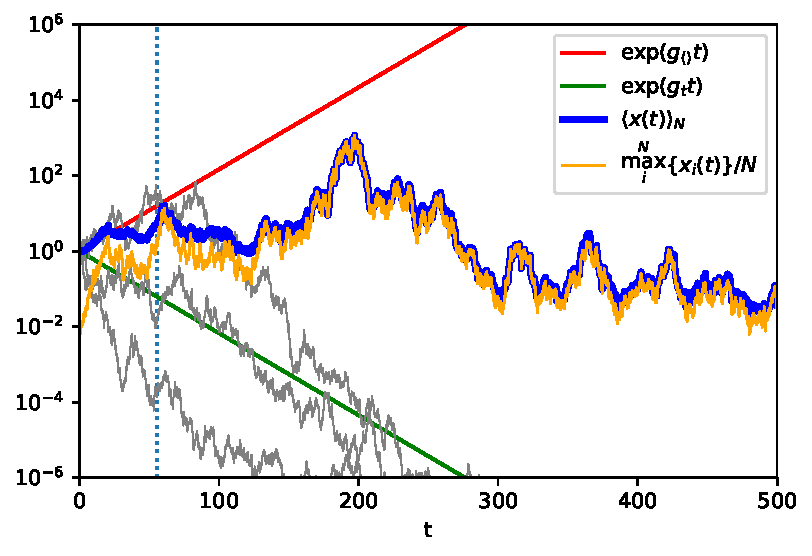
\includegraphics[height=9.3cm]{./chapter_3/figs/trajectories.pdf}
\caption{PEA and maximum in a finite ensemble of size $\N=256$. {\bf \underline{Red line:}} expectation value $\ave{\x(\t)}$. 
{\bf \underline{Green line:}} exponential growth at the time-average growth rate. In the $\t\to\infty$ limit all trajectories grow at this rate. 
{\bf \underline{Yellow line:}} contribution of the maximum value of any trajectory at time $\t$ to the PEA.  
{\bf \underline{Blue line:}} PEA $\ave{\x(\t)}_\N$.
{\bf \underline{Vertical line:}} Crossover -- for $\t>\t_c=\frac{2\ln \N}{\gsigma^2}$ the maximum begins to dominate the PEA (the yellow line approaches the blue line).
{\bf \underline{Grey lines:}} randomly chosen trajectories -- any typical trajectory soon grows at the time-average growth rate.  
{\bf \underline{Parameters:}} $\N=256$, $\gmu=0.05$, $\gsigma=\sqrt{0.2}$.}
\flabel{trajectories}
\end{figure}
\FloatBarrier

In \cite{PetersKlein2013} we analysed PEAs of \GBM analytically and numerically. Using \eref{GBM_sol} the PEA can be written as
\be
\ave{\x}_\N=\frac{1}{\N} \sum_{i=1}^\N \exp\left[ \left(\gmu-\frac{\gsigma^2}{2}\right) \t + \gsigma \gW_i(\t) \right],
\elabel{PEA}
\ee
where $\left\{\gW_i(\t)\right\}_{i=1\dots \N}$ are $\N$ independent realisations of the Wiener process. Taking the deterministic part out of the sum, we can write
\be
\ave{\x}_\N=\exp\left[ \left(\gmu-\frac{\gsigma^2}{2}\right) \t \right] \frac{1}{\N} \sum_{i=1}^\N \exp\left(\t^{1/2} \gsigma \xi_i\right),
\elabel{PEA_2}
\ee
where $\left\{\xi_i\right\}_{i=1\dots \N}$ are $\N$ independent standard normal variates.

We found that typical trajectories of PEAs grow at $\gex$ up to a time $t_c$ 
that is logarithmic in $\N$, meaning $\t_c\propto \ln \N$. This is consistent with our analytical sketch. After this time, typical 
PEA trajectories begin to deviate from expectation-value behaviour, and eventually 
their growth rate converges to $g_t$. While the two limiting behaviours $\N\to\infty$
and $\t\to \infty$ can be computed exactly, what happens in between
is less straightforward. The PEA is a random object outside these limits. 

A quantity of crucial interest to us is the exponential growth rate experienced by the PEA, 
\be
\gest(\t,\N) \equiv \frac{\ln(\ave{\x(\t)}_\N)- \ln(\x(0))}{\t-0} = \frac{1}{\t}\ln(\ave{\x(\t)}_\N).
\elabel{g_est}
\ee
In \cite{PetersKlein2013} we proved that the $\t\to\infty$ limit for any (finite) 
$\N$ is the same as for the case $\N=1$, 
\be
\lim_{\t\to\infty}\gest(\t,\N)=\gmu-\frac{\gsigma^2}{2}
\elabel{gest_2}
\ee
for all $\N\geq1$. Substituting \eref{PEA_2} in \eref{g_est} produces
\bea
\gest(\t,\N)&=&\gmu-\frac{\gsigma^2}{2}+\frac{1}{\t} \ln\left(\frac{1}{\N} \sum_{i=1}^\N \exp( \t^{1/2} \gsigma \xi_i)\right)\\
&=&\gmu-\frac{\gsigma^2}{2}-\frac{\ln \N}{\t}+\frac{1}{\t} \ln\left(\sum_{i=1}^\N \exp( \t^{1/2} \gsigma \xi_i)\right).
\elabel{gest_4}
\eea

We didn't look in \cite{PetersKlein2013} at the expectation value of $\gest(\t,\N)$ for finite time and finite samples, but it's an interesting object that depends on $\N$ and $\t$ but is not stochastic. Note that this is not $\gest$ of the expectation value, 
which would be the $\N\to\infty$ limit of \eref{g_est}. Instead it is the 
$S\to\infty$ limit,
\be
\ave{\gest(\t,\N)} = \frac{1}{\t}\ave{\ln(\ave{\x(\t)}_\N)} = f(\N,\t),
\elabel{gest_3}
\ee
where, as previously, $\ave{\cdot}$ without subscript refers to the average over all possible samples, \ie $\lim_{S\to\infty}\ave{\cdot}_{S}$. The last two terms in \eref{gest_4} suggest an exponential relationship between ensemble size and time. The final term is a tricky stochastic object on which the properties of the expectation value in \eref{gest_3} will hinge. This term will be the focus of our attention: the sum of exponentials of normal random variates or, equivalently, log-normal variates.

\subsubsection{The random energy model}
\seclabel{REM}
Since the publication of \cite{PetersKlein2013} we have learned, thanks to discussions with J.-P.~Bouchaud, 
that the key object in \eref{gest_4} -- the sum log-normal random variates -- has been of
interest to the mathematical physics community since the 1980s. The reason for this is Derrida's random energy model \cite{Derrida1980,Derrida1981}, which we will describe here. This section is very ``physicsy'' and the key results are in \eref{gest_7} and \eref{gest_8} -- it's safe to skip to them, if you like.

The model is defined as follows. Imagine a system whose energy levels are $2^K=\N$ normally-distributed random numbers, $\xi_i$ (corresponding to $K$ spins). This is a very simple model of a disordered system, such as a spin glass, the idea being that the system is so complicated that we ``give up'' and simply model its energy levels as realisations of a random variable. (We denote the number 
of spins by $K$ and the number of resulting energy levels by $\N$, while Derrida uses $\N$ for the number of spins). The partition function is then
\be
Z=\sum_{\gi=1}^\N \exp\left(\beta J\sqrt{\frac{K}{2}}\xi_\gi\right),
\elabel{Z}
\ee
where the inverse temperature, $\beta$, is measured in appropriate units, and the scaling in $K$ is chosen
so as to ensure an extensive thermodynamic limit \cite[p.~79]{Derrida1980}. $J$ is a constant that will be determined below.
The logarithm of the partition function gives the Helmholtz free energy, 
\bea
F&=&-\frac{\ln Z}{\beta}\\
&=&-\frac{1}{\beta}  \ln\left[\sum_{\gi=1}^\N \exp\left(\beta J \sqrt{\frac{K}{2}}\xi_\gi\right)\right].
\elabel{F}
\eea

Like the growth rate estimator in \eref{g_est}, this involves a sum of 
log-normal variates and, indeed, we can rewrite \eref{gest_4} as
\be
\gest=\gmu-\frac{\gsigma^2}{2}-\frac{\ln \N}{\t}-\frac{\beta F}{\t},
\elabel{gest_5}
\ee
which is valid provided that
\be
\beta J \sqrt{\frac{K}{2}}=\gsigma \t^{1/2}.
\elabel{map}
\ee
\Eref{map} does not give a unique mapping between the parameters of our \GBM, $(\gsigma, \t)$, and the parameters of the REM, $(\beta, K, J)$. Equating (up to multiplication) the constant parameters, $\gsigma$ and $J$, in each model gives us a specific mapping:
\be
\gsigma=\frac{J}{\sqrt{2}} \quad \text{and} \quad \t^{1/2} = \beta\sqrt{K}.
\elabel{choice_1}
\ee

The expectation value of $\gest$ is interesting. The only random object
in \eref{gest_5} is $F$. Knowing $\ave{F}$ thus amounts to knowing $\ave{\gest}$.
In the statistical mechanics of the random energy model, $\ave{F}$ is of key
interest and so much about it is known. We can use this knowledge
thanks to the mapping between the two problems.

Derrida identifies a critical temperature,
\be
\frac{1}{\beta_c} \equiv \frac{J}{2\sqrt{\ln 2}},
\elabel{beta_c}
\ee
above and below which the expected free energy scales differently with $K$ and $\beta$. This maps to a critical time scale in \GBM,
\be
\t_c = \frac{2\ln \N}{\gsigma^2},
\elabel{t_c}
\ee
with high temperature ($1/\beta>1/\beta_c$) corresponding to short time ($\t<\t_c$) and low temperature ($1/\beta<1/\beta_c$) corresponding to long time ($\t>\t_c$). Note that $t_c$ in \eref{t_c} scales identically with $\N$ and $\gsigma$ as the transition time, \eref{short_t}, in our sketch.

In \cite{Derrida1980}, $\ave{F}$ is computed in the high-temperature (short-time) regime as
\bea
\ave{F}&=&E-S/\beta \\
&=&-\frac{K}{\beta} \ln2 - \frac{\beta K J^2}{4},
\elabel{F_2}
\eea
and in the low-temperatures (long-time) regime as
\be
\ave{F}=-KJ\sqrt{\ln 2}.
\elabel{F_3}
\ee

\paragraph{\underline{Short time}}
\mbox{}

We look at the short-time behavior first (high $1/\beta$, \eref{F_2}).
The relevant computation of the entropy $S$ in \cite{Derrida1980} 
involves replacing the number of energy levels
$\N(E)$ by its expectation value $\ave{\N(E)}$. This is justified because
the standard deviation of this number is $\sqrt{\N}$ and relatively small
when $\ave{\N(E)}>1$, which is the interesting regime in Derrida's case. 

For spin glasses, the expectation value of $F$ is interesting, supposedly, 
because the system may be self-averaging and can be thought of as an
ensemble of many 
smaller sub-systems that are essentially independent. The macroscopic
behavior is then given by the expectation value.

Taking expectation values and substituting from \eref{F_2} in \eref{gest_5} we find
\be
\ave{\gest}^{\text{short}}=\gmu-\frac{\gsigma^2}{2}+\frac{1}{\t} \frac{K J^2}{4T^2}.
\elabel{gest_6}
\ee
From \eref{map} we know that $\t=\frac{KJ^2}{2\gsigma^2T^2}$, which we substitute to find
\be
\ave{\gest}^{\text{short}}=\gmu.
\elabel{gest_7}
\ee
This is the correct behavior in the short-time regime.

\paragraph{\underline{Long time}}
\mbox{}

Next, we turn to the expression for the long-time regime (low temperature, \eref{F_3}). 
Again 
taking expectation values and substituting, this time from \eref{F_3} in \eref{gest_5}, we find
for long times
\be
\ave{\gest}^{\text{long}}=\gmu-\frac{\gsigma^2}{2}-\frac{\ln{\N}}{\t}+\sqrt{\frac{2\ln \N}{\t}}\,\gsigma,
\elabel{gest_8}
\ee
which has the correct long-time asymptotic behavior.
The form of the correction to the time-average growth rate
in \eref{gest_8} is consistent with \cite{PetersKlein2013} and \cite{Redner1990}, where
it was found that approximately $\N=\exp(\t)$ systems are required for ensemble-average
behavior to be observed for a time $\t$, so that the parameter $\ln \N/\t$ controls
which regime dominates. If the parameter is small, then \eref{gest_8} indicates that the
long-time regime is relevant.

\Fref{1} is a direct comparison between the results derived
here, based on \cite{Derrida1980}, and numerical results using the same parameter 
values as in \cite{PetersKlein2013}, namely $\gmu=0.05, \gsigma=\sqrt{0.2}, \N=256$ and $S=10^5$.

Notice that $\ave{\gest}$ is not the (local)
time derivative $\frac{\partial}{\partial \t}\ave{\ln(\ave{\x}_\N)}$, but a time-average growth rate, $\ave{\frac{1}{\t}\ln\left( \frac{\ave{\x(\t)}_\N}{\ave{\x(0)}_\N}\right)}$. It is remarkable that the expectation value $\ave{\gest(\N,\t)}$ so closely reflects the
median, $q_{0.5}$, of $\ave{\x}_\N$, \ie
\be
q_{0.5}(\ave{\x(\t)}_\N) \approx \exp \left(\ave{\gest(\N,\t)}\t\right).
\elabel{quant_ave}
\ee
In \cite{PetersGell-Mann2016} it was discussed in detail that 
$\gest(1,\t)$ is an ergodic observable for \eref{GBM}, in the sense that 
$\ave{\gest(1,\t)}=\lim_{\t\to\infty} \gest$. The relationship in \eref{quant_ave}
is far more subtle. The typical behavior of \GBM PEAs 
is complicated outside the limits $\N\to\infty$ or $\t\to\infty$, where growth rates are time-dependent. This complicated behaviour is well represented by an 
approximation that uses physical insights into spin glasses.

\begin{figure}
\centering
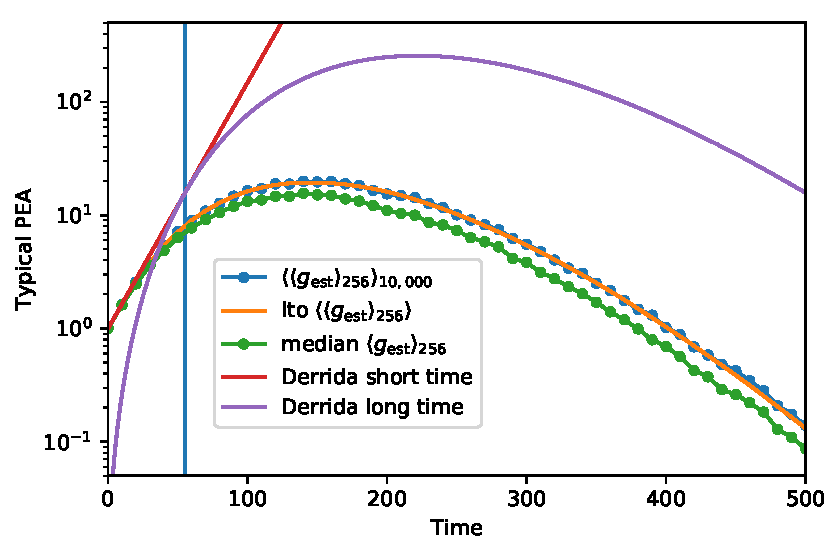
\includegraphics[height=9.3cm]{./chapter_3/figs/PEA.pdf}
\caption{Lines are obtained by exponentiating the various exponential 
growth rates. {\bf \underline{Blue line:}} $\ave{\ave{\gest}_{256}}_{10,000}$ is the numerical mean 
(approximation of the expectation value) 
over a super-ensemble of $S=10,000$ samples of $\gest$ estimated in sub-ensembles of $\N=256$ GBMs each. 
{\bf \underline{Green line:}} median in a super-ensemble of $S$ samples of $\gest$, each estimated in sub-ensembles of size $\N$. 
{\bf \underline{Yellow line:}} An exact expression for $d\ave{\ln\ave{\x}_\N}$, derived using \Ito calculus, see \cite{PetersAdamou2018b}. We evaluate the expression by Monte Carlo, and integrate, $\ave{\ln\ave{\x}_\N}=\int_{0}^{\t} d\ave{\ln\ave{\x}_\N}$. Exponentiation yields the yellow line. 
{\bf \underline{Red line:}} short-time behavior, based on the random energy model, \eref{gest_7}.
{\bf \underline{Purple line:}} long-time behavior, based on the random energy model, \eref{gest_8}. {\bf \underline{Vertical line:}} Crossover between the regimes at $t_c=\frac{2\ln \N}{\gsigma^2}$, corresponding to $\beta_c=\frac{2(\ln 2)^{1/2}}{J}$.
{\bf \underline{Parameters:}} $\N=256$, $S=10,000$, $\gmu=0.05$, $\gsigma=\sqrt{0.2}$.}
\flabel{1}
\end{figure}
\FloatBarrier

\newpage

%%%%%%%%%%%%%%%%%%%%%%%%%%%%%%%%%%%%%%%
%% NEW CHAPTER
%%%%%%%%%%%%%%%%%%%%%%%%%%%%%%%%%%%%%%%

\section{Interactions}
{\it
We add interactions to our null model of a population of noisy multipliers. It turns out that our decision criterion generates interesting emergent behaviour -- cooperation, the sharing and pooling of resources, is often time-average 
growth optimal. This provides answers to the puzzles of why people cooperate and why we see socio-economic structure from the formation of firms to nation states with taxation and redistribution systems. We also ask whether assumptions about ergodicity in standard treatments of these topics are justified.}
\newpage


%%%%%%%%%%%%%%%%%%%%%%%%%%%%%%%%%%%%%%%

\subsection{Cooperation}
\seclabel{Cooperation}
Under multiplicative growth, fluctuations are undesirable because they reduce 
time-average growth rates. In the long run, wealth $\x_1(\t)$ with noise term 
$\gsigma_1$ will outperform wealth $\x_2(\t)$ with a larger 
noise term $\gsigma_2>\gsigma_1$, in the sense that 
\be
\gt(\x_1) > \gt(\x_2)
\ee
with probability 1.

For this reason it is desirable to reduce fluctuations. One protocol that achieves this is pooling and sharing of resources. In \secref{Every_man} we explored the world created 
by the model of independent GBMs. This is a world where everyone experiences the 
same long-term growth rate. We want to explore the effect of the invention of 
cooperation. It turns out that cooperation increases growth rates, and this is a 
crucial insight. 

Suppose two individuals, $\x_1(\t)$ and $\x_2(\t)$ decide to meet up every Monday, put all their wealth on a table, divide it in two equal amounts, and go back to their business (where their business is making their wealths follow \GBM!) How 
would this operation affect the dynamic of the wealth of these two individuals?

Consider a discretised version of \eref{GBM}, such as would be used in a numerical simulation. The non-cooperators grow according to
 \bea
 \D \x_\gi(\t) & = & \x_\gi(\t) \left[\gmu \D\t + \gsigma \sqrt{\D\t}\,\xi_i\right], \elabel{discrete_nonc_grow} \\
 \x_\gi(\t+\D\t) & = & \x_\gi(\t) + \D \x_\gi(\t), \elabel{discrete_nonc_coop}
 \eea
 where $\xi_i$ are standard normal random variates, $\xi_i\sim \mathcal{\N}(0,1)$.

We imagine that the two previously non-cooperating entities, with resources $\x_1(\t)$ and $\x_2(\t)$, cooperate to produce two entities, whose resources we label $\x^c_1(\t)$ and $\x^c_2(\t)$ to distinguish them from the non-cooperating case. We envisage equal sharing of resources, $\x^c_1=\x^c_2$, and introduce a cooperation operator, $\oplus$, such that
 \be
 \x_1 \oplus \x_2 = \x^c_1 + \x^c_2.
 \ee
 
 In the discrete-time picture, each time step involves a two-phase process. First there is a growth phase, analogous to \eref{GBM}, in which each cooperator increases its resources by
 \be
 \D \x^c_\gi(\t) = \x^c_\gi(\t)\left[\gmu\D\t + \gsigma\sqrt{\D\t}\,\xi_\gi\right].
 \elabel{discrete_coop_grow}
 \ee
 This is followed by a cooperation phase, replacing \eref{discrete_nonc_coop}, in which resources are pooled and shared equally among the cooperators:
 \be
 \x^c_\gi(\t+\D\t) = \frac{ \x^c_1(\t) + \D \x^c_1(\t) + \x^c_2(\t) + \D \x^c_2(\t)}{2}.
 \elabel{discrete_coop_coop}
 \ee
 
 \begin{figure}
 \centering
 \begin{picture}(300,230)(60,0)
 \put(-20,0){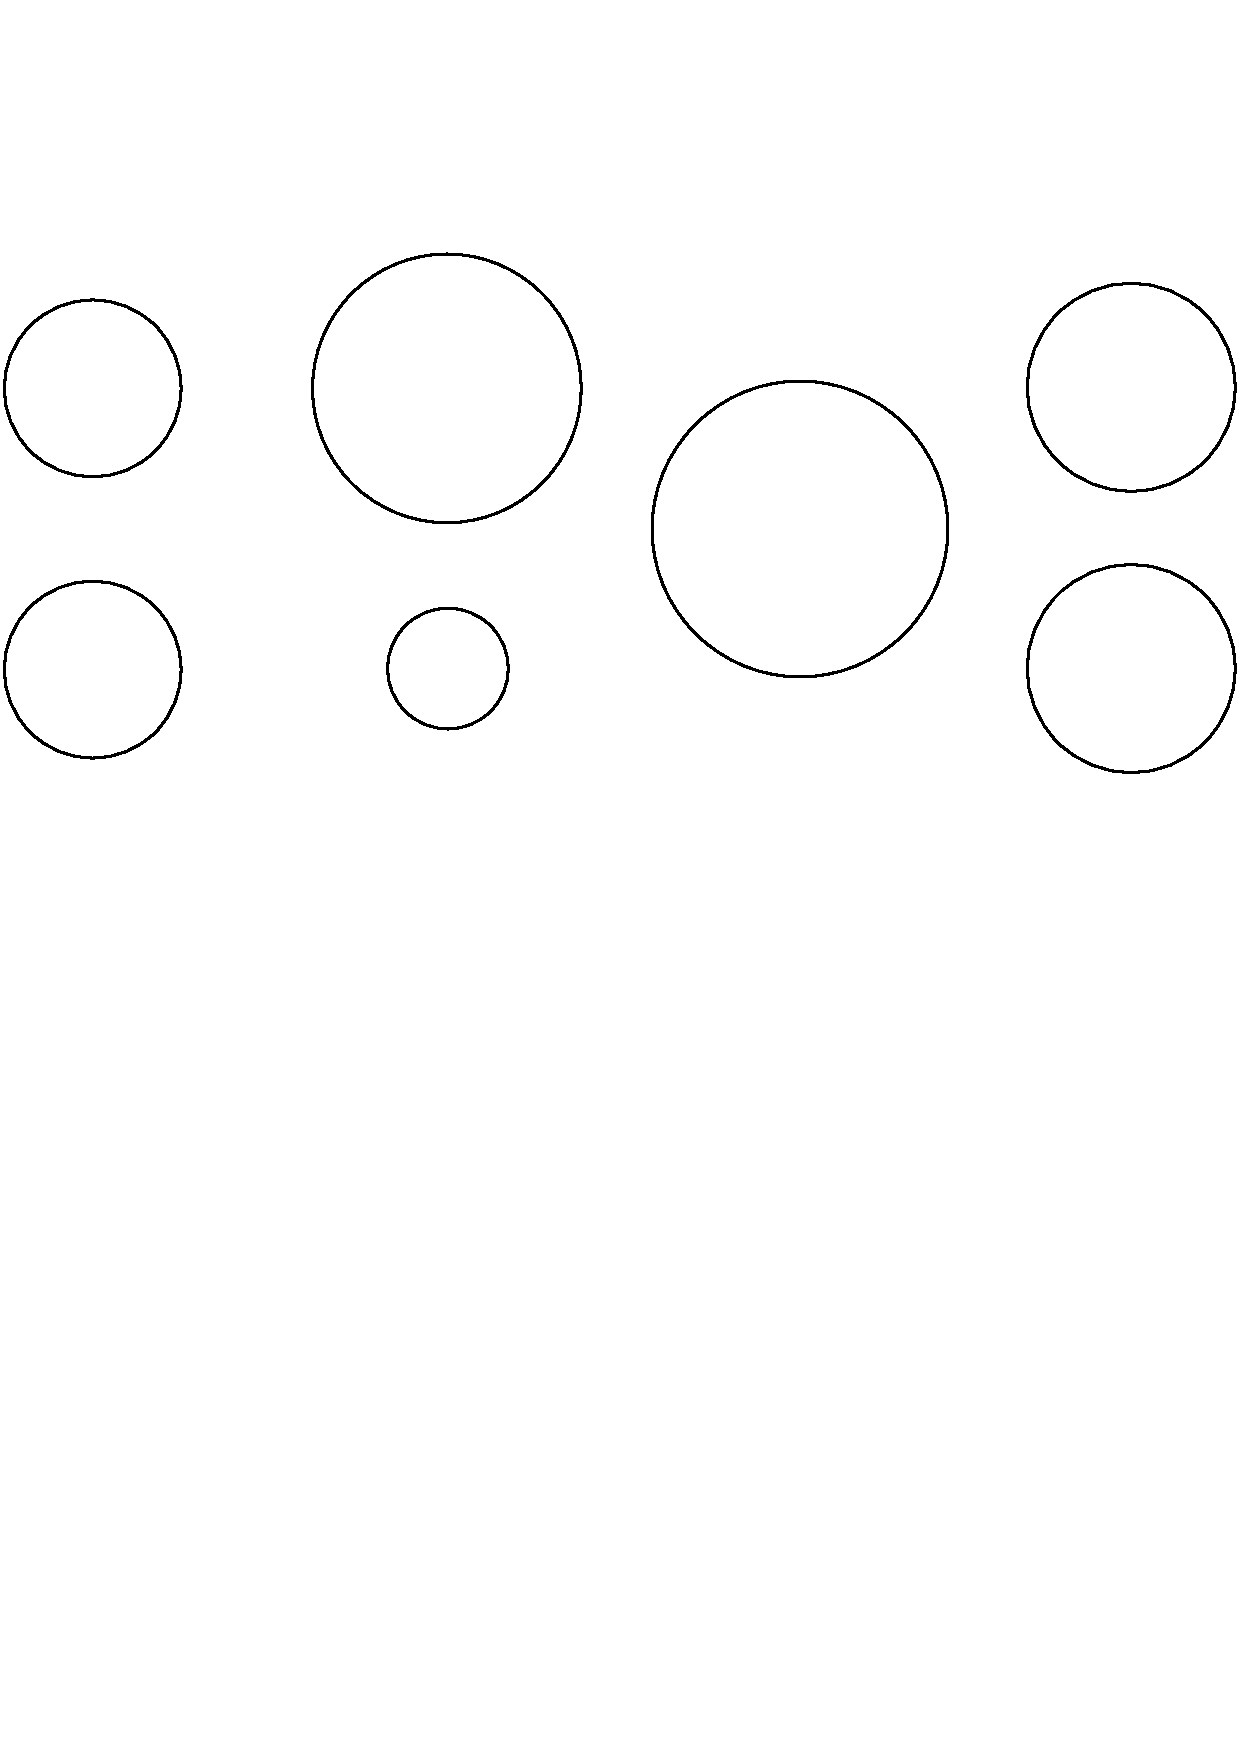
\includegraphics[width=470pt]{./chapter_3/figs/blobs.pdf}}
 \put(0,145){$\x^c_1(\t)$}
 \put(48,147){\vector(1,0){45}}
 \put(0,40){$\x^c_2(\t)$}
 \put(48,40){\vector(1,0){75}}
 %
 \put(115,145){$\x^c_1(\t)+\D \x^c_1(\t)$}
 \put(200,147){\vector(3,-2){30}}
 \put(138,46){$\x^c_2(\t)$}
 \put(130,34){$+\D \x^c_2(\t)$}
 \put(173,45){\vector(3,2){50}}
 %
 \put(255,100){$\x^c_1(\t)+\D \x^c_1(\t)$}
 %
 \put(250,85){$+ \x^c_2(\t)+\D \x^c_2(\t)$}
 \put(335,75){\vector(3,-2){30}}
 \put(335,117){\vector(3,2){30}}
 %
 \put(385,145){$\x^c_1(\t+\D\t)$}
 \put(385,40){$\x^c_2(\t+\D\t)$}
 %
 \put(448,147){\vector(1,0){25}}
 \put(448,40){\vector(1,0){25}}

 \put(476,144.5){$\cdots$}
 \put(476,37.5){$\cdots$}
 % AA extra arrows
 \put(-47,117){\vector(3,2){25}}
 \put(-47,75){\vector(3,-2){25}}
 \put(-62,114){$\cdots$}
 \put(-62,73){$\cdots$}
 %
 \put(50,207.5){\large{Grow}}

 \put(215,190){$\overbrace{\text{Pool} \hspace{3cm}\text{Share}}^{\text{\large{Cooperate}}}$}

 \end{picture}
 \caption{Cooperation dynamics. Cooperators start each time step with equal resources, then they {\it grow} independently 
 according to \eref{discrete_coop_grow}, then they {\it cooperate} by {\it pooling} resources and {\it sharing} them equally, 
 then the next time step begins. 
  }
 \flabel{dynamics}
 \end{figure}
 

 %Analysis
 With this prescription both cooperators and their sum experience the following dynamic:
 \be
 (\x_1 \oplus \x_2)(\t+\D\t) =
 (\x_1 \oplus \x_2)(\t) \left[1 + \left(\gmu \D\t + \gsigma \sqrt{\D\t} \, \frac{\xi_1 + \xi_2}{2}\right)\right].
 \elabel{discrete_cooperate}
 \ee
 For ease of notation we define
 \be
 \xi_{1\oplus2}=\frac{\xi_1+\xi_2}{\sqrt{2}},
 \ee
 which is another standard Gaussian, $\xi_{1\oplus2} \sim \mathcal{\N}(0,1)$. Letting the time
 increment $\D\t \to 0$ we recover an equation of the same form as
 \eref{GBM} but with a different fluctuation amplitude,
 \begin{equation}
 \gd(\x_1 \oplus \x_2) = (\x_1 \oplus \x_2)\left(\gmu \gd\t +\frac{\gsigma}{\sqrt{2}} \gd\gW_{1\oplus2}\right).
 \end{equation}
 
The expectation values of a non-cooperator, $\ave{\x_1(\t)}$, and a corresponding cooperator,
$\ave{\x^c_1(\t)}$, are identical. Based on expectation values, we thus cannot 
 see any benefit of cooperation. Worse still, immediately after the growth phase, the 
 better-off entity of a cooperating pair, $\x^c_1(t_0)>\x^c_2(t_0)$, say, would increase its expectation value from 
$\frac{\x^c_1(t_0)+\x^c_2(t_0)}{2}\exp(\gmu (\t-t_0))$ to $\x^c_1(t_0)\exp(\gmu (\t-t_0))$
by breaking the cooperation. But it would be foolish to act on the basis of this analysis:
the short-term gain from breaking cooperation is a one-off, and is dwarfed by the long-term
multiplicative advantage of continued cooperation. 
An analysis based on expectation values finds that there is no reason for 
cooperation to arise, and that if it does arise there are good reasons for it to end, 
\ie it will be fragile. Because expectation values are inappropriately used to evaluate 
future prospects, the observation of widespread cooperation constitutes a conundrum. 

%Solution of the cooperation conundrum
The solution of the conundrum comes from considering the time-average
growth rate. The non-cooperating entities grow at $g_{\t}(\x_\gi)=\gmu-\frac{\gsigma^2}{2}$, 
whereas the cooperating unit benefits from a reduction of the amplitude of relative 
fluctuations and grows at $g_{\t}(\x_1\oplus \x_2)=\gmu-\frac{\gsigma^2}{4}$, 
and we have
\begin{equation}
g_{\t}(\x_1\oplus \x_2)>g_{\t}(\x_\gi)
\end{equation}
for any non-zero noise amplitude. Imagine a world where cooperation does not exist, 
just like in \secref{Every_man}. Now introduce into this world two individuals who have 
invented cooperation -- very quickly this pair of individuals will become vastly more wealthy than
anyone else. To keep up, others will have to start cooperating. The effect is illustrated 
in \fref{cooperate} by direct simulation of
\eref{discrete_nonc_grow}--\eref{discrete_nonc_coop} and \eref{discrete_cooperate}.

\begin{figure}
\begin{picture}(200,300)(0,0)
\put(-35,-135){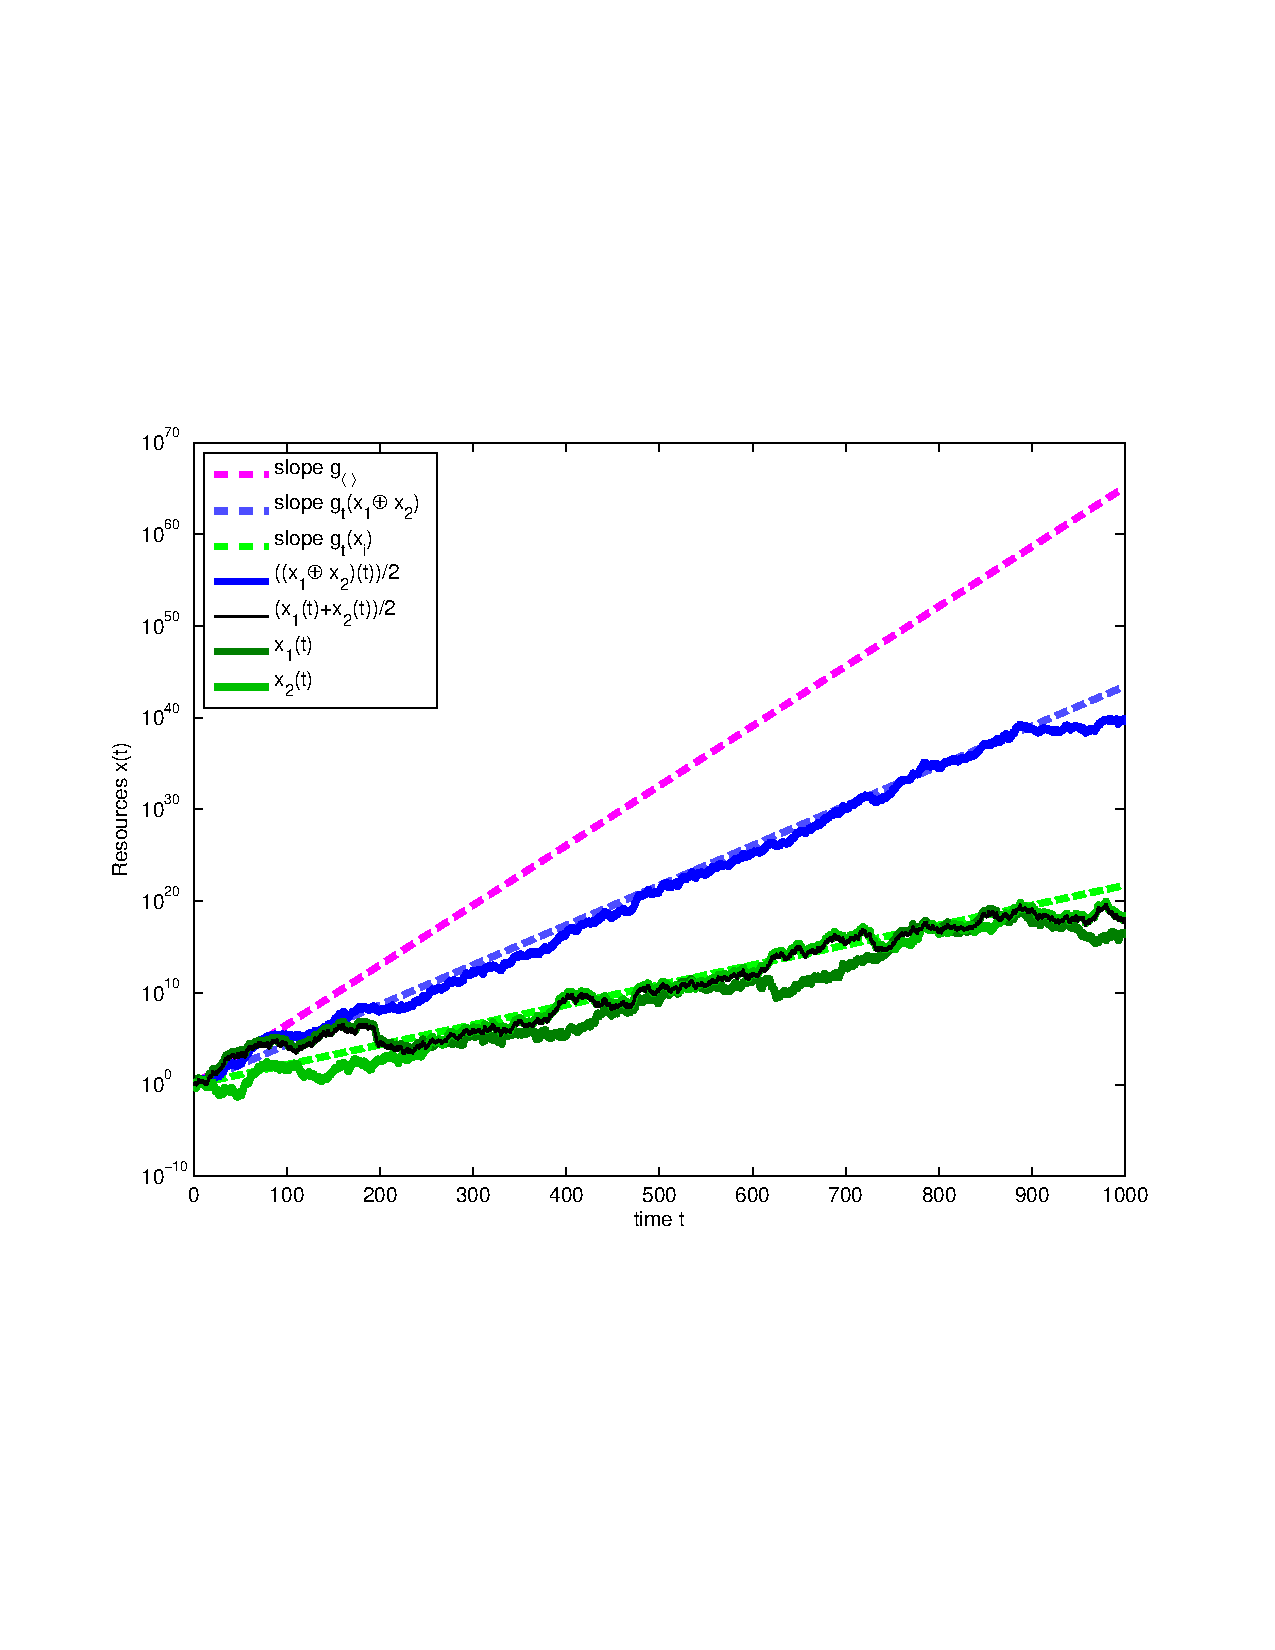
\includegraphics[width=440pt]{./chapter_3/figs/cooperate.pdf}}
\end{picture}
\caption{Typical trajectories for two non-cooperating (green) entities and for the 
corresponding cooperating unit (blue).
Over time, the noise reduction for the cooperator leads to faster growth. Even without
effects of specialisation or the emergence of new function, 
cooperation pays in the long run. The black thin line shows the average of the 
non-cooperating entities. While in the logarithmic vertical scale the average traces
the more successful trajectory, it is far inferior to the cooperating unit. 
In a very literal mathematical sense the whole, $(\x_1 \oplus \x_2)(\t)$, is more than the sum of its
parts, $\x_1(\t)+\x_2(\t)$. The algebra of cooperation is not merely that of summation.}
\flabel{cooperate}
\end{figure}

Imagine again the pair of cooperators outperforming all of their peers. Other
entities will have to form pairs to keep up, and the obvious next step is for larger
cooperating units to form -- groups of 3 may form, pairs of pairs, cooperation 
clusters of $\N$ individuals, and the larger the cooperating group the closer the
time-average growth rate will get to the expectation value.
For $\N$ cooperators, $\x_1\oplus \x_2 ... \oplus \x_\N$ the spurious drift term is 
$-\frac{\gsigma^2}{2\N}$, so that the time-average growth approaches 
expectation-value growth for large $\N$. The approach to this upper bound as 
the number of cooperators increases favours the formation of social structure. 

We may generalise to different drift 
terms, $\gmu_\gi$, and noise amplitudes, $\gsigma_\gi$, for different individual entities. 
Whether cooperation is beneficial in the long run for any
given entity depends on these parameters as follows. Entity 1 
will benefit from cooperation with entity 2 if 
\be
\gmu_1-\frac{\gsigma_1^2}{2}<\frac{\gmu_1+\gmu_2}{2}-\frac{\gsigma_1^2+\gsigma_2^2}{8}.
\ee
We emphasize that this inequality may be satisfied also if the expectation value
of entity 1 grows faster than the expectation value of entity 2, \ie if
$\gmu_1>\gmu_2$. An analysis of expectation values, again, is utterly misleading:
the benefit conferred on entity 1 due to the fluctuation-reducing effect of 
cooperation may outweigh the cost of having to cooperate with an entity with
smaller expectation value.

We may also generalise to correlations between the fluctuations experienced by different entities. These are uncorrelated in our model: the $\gd\gW_\gi$ in \eref{GBM} and, consequently, the $\xi_\gi$ in \eref{discrete_nonc_grow} onwards are independent random variables. In reality, cooperators are often spatially localised and experience similar environmental conditions. By allowing correlations between the $\xi_i$, our model can be adapted to describe such situations. This is more technically difficult and we won't present it here. If you are interested, you can find the details in \cite{PetersAdamou2015a}.
 
Notice the nature of the Monte-Carlo simulation in \fref{cooperate}. No ensemble
is constructed. Only individual trajectories are simulated and run for a time that is 
long enough for statistically significant features to rise above the noise. This method
teases out of the dynamics what happens over time. The significance of any observed 
structure -- its epistemological meaning -- is immediately clear: this is what happens over time
for an individual system (a cell, a person's wealth, {\it etc.}). Simulating an ensemble
and averaging over members to remove noise does not tell the same story. The resulting
features may not emerge over time. They are what happens on average in an ensemble, 
but -- at least for \GBM -- this is not what happens to the individual with probability 1. For instance the 
 pink dashed line in \fref{cooperate} is the ensemble average of $\x_1(\t)$, $\x_1(\t)$, 
 and $(\x_1 \oplus \x_2)(\t)/2$, and it has nothing to do with what happens 
 in the individual trajectories over time.

When judged on expectation values, the apparent futility of cooperation is unsurprising
because expectation values are the result for infinitely 
many cooperators, and adding further cooperators cannot improve on this.

In our model the advantage of cooperation, and hence the emergence
of social structure in the broadest sense -- is purely a non-linear 
effect of fluctuations -- cooperation reduces the magnitude of 
fluctuations, and over time (though not in expectation) this implies faster growth. 


Another generalisation is partial cooperation -- entities may share only
a proportion of their resources, resembling taxation and redistribution. We discuss this in the next section.

%%%%%%%%%%%%%%%%%%%%%%%%%%%%%%%%%%%%%%%

\subsection{Reallocation}
\seclabel{reallocation}

%%%%%%%%%%%%%%%%%%%%%%%%%%%%%%%%%%%%%%%

\subsubsection{Introduction}
\seclabel{RGBM_intro}

In \secref{Every_man} we created a model world of independent trajectories of \GBM. We studied how the distribution of the resulting random variables evolved over time. We saw that this is a world of broadening distributions, increasing inequality, and wealth condensation.

We introduced cooperation to it in \secref{Cooperation} and saw how this increases the time-average growth rate for those who pool and share all of their resources. In this section we study what happens if a large number of individuals pool and share only a fraction of their resources. This is reminiscent of the taxation and redistribution -- which we shall call ``reallocation'' -- carried out by populations in the real world.

We will find that, while full cooperation between two individuals increases their growth rates, sufficiently fast reallocation from richer to poorer in a large population has two related effects. Firstly, everyone's wealth grows in the long run at a rate close to that of the expectation value. Secondly, the distribution of rescaled wealth converges over time to a stable form. This means that, while wealth can still be distributed quite unequally, wealth condensation and the divergence of inequality no longer occur in our model. Of course, for this to be an interesting finding, we will have to quantify what we mean by ``sufficiently fast reallocation.''

We will also find that when reallocation is too slow or, in particular, when it goes from poorer to richer -- which we will label negative reallocation -- no stable wealth distribution exists. In the latter case, the population splits into groups with positive and negative wealths, whose magnitudes grow exponentially.

Finally, having understood how our model behaves in each of these reallocation regimes, we will fit the model parameters to historical wealth data from the real world, specifically the United States. This will tell us which type of model behaviour best describes the dynamics of the US wealth distribution in both the recent and more distant past. You might find the results surprising -- we certainly did!

%%%%%%%%%%%%%%%%%%%%%%%%%%%%%%%%%%%%%%%

\subsubsection{The ergodic hypothesis in economics}
\seclabel{RGBM_EH}
% Introduce the EH
Of course, we are not the first to study resource distributions and inequality in economics. This topic has a long history, going back at least as far as Vilfredo Pareto's work in the late $19^\text{th}$ century \cite{Pareto1897} (in which he introduced the power-law distribution we discussed in \secref{power_law}). It's worth spending a few moments considering how the subject is approached classically, before we say how we approach it.

Economists studying such distributions usually make the following assumption in their models: that the distributions converge in the long run to a unique and stable form, regardless of initial conditions. This allows them to study the stable distribution, for which many statistical techniques exist, and to ignore the transient phenomena preceding it, which are far harder to analyse. Paul Samuelson called this the ``ergodic hypothesis'' \cite[pp.~11-12]{Samuelson1968}. It's easy to see why: if this convergence happens, then the time average of the observable under study will equal its ensemble average with respect to the stable distribution.\footnote{Convergence to a unique and stable distribution is a sufficient but not necessary condition for an ergodic observable, as we have defined it.}

% Transformation is needed
Economics is often concerned with growth and a growing quantity cannot be ergodic in Samuelson's sense, because its distribution never stabilises. This suggests the simplifying ergodic hypothesis should \textit{never} be made. Not so fast! Although rarely stated, a common strategy to salvage these techniques is to find a transformation of the non-ergodic process that produces a meaningful ergodic observable. If such an ergodic observable can be derived, then classical analytical techniques may still be used. We have already seen in the context of gambles that expected utility theory can be viewed as transformation of non-ergodic wealth increments into ergodic utility increments. Expectation values, which would otherwise be misleading, then quantify time-average growth of the decision-maker's wealth.

% This is done in studies of wealth distributions
Studies of wealth distributions also employ this strategy. Individual wealth is modelled as a growing quantity. Dividing by the population average transforms this to a rescaled wealth, as in \secref{rescaled}, which is hypothesised to be ergodic. For example, \cite[p.~130]{BenhabibBisinZhu2011} ``impose assumptions \dots that guarantee the existence and uniqueness of a limit stationary distribution.'' The idea is to take advantage of the simplicity with which the stable distribution can be analysed, \eg to predict the effects of policies encoded in model parameters.

% What is the problem? What are we going to do?
There is, however, an elephant in the room. To our knowledge, the validity of the ergodic hypothesis for rescaled wealth has never been tested empirically. It's certainly invalid for the \GBM model world we studied previously because, as we saw in \secref{rescaled}, rescaled wealth has an ever-broadening log-normal distribution. That doesn't seem to say much, as most reasonable people would consider our model world -- containing a population of individuals whose wealths multiply noisily and who never interact -- a tad unrealistic. The model we are about to present will not only extend our understanding from this simple model world to one containing interactions, but also will allows us to test the hypothesis. This is because it has regimes, \ie combinations of parameters, for which rescaled wealth is and isn't ergodic. This contrasts with models typically used by economists, which have the ergodic hypothesis ``baked in.''

% Convergence time
If it is reasonable to assume a stable distribution exists, we must also consider how long convergence to would take after a change of parameters. It's no use if convergence in the model takes the whole of human history, if we are using it to estimate the effect of a tax policy over the next election cycle. Therefore, treating a stable model distribution as representative of an empirical wealth distribution implies an assumption of fast convergence.  As the late Tony Atkinson pointed out, ``the speed of convergence makes a great deal of difference to the way in which we think about the model'' \cite{atkinson1969timescale}. We will use our model to discuss this point. Without further ado, let us introduce it.

%%%%%%%%%%%%%%%%%%%%%%%%%%%%%%%%%%%%%%%

\subsubsection{Reallocating geometric Brownian motion}
\seclabel{RGBM_model}
% model
Our model, called \RGBM, is a system of $\N$ individuals whose wealths, $\x_\gi(\t)$, evolve according to the stochastic differential equation,
\be
\gd\x_\gi=\x_\gi \left[(\gmu-\gphi)\gd\t+\gsigma \gd\gW_\gi\left(\t\right)\right]+ \gphi\ave{\x}_\N\gd\t,
\elabel{rgbm}
\ee
for $\gi=1\dots \N$. In effect, we have added to \GBM a simple reallocation mechanism. Over a time step, $dt$, each individual pays a fixed proportion of its wealth, $\gphi \x_\gi \gd\t$, into a central pot (``contributes to society'') and gets back an equal share of the pot, $\gphi\ave{\x}_\N \gd\t$, (``benefits from society''). We can think of this as applying a wealth tax, say of $1\%$ per year, to everyone's wealth and then redistributing the tax revenues equally. Note that the reallocation parameter, $\gphi$, is, like $\gmu$, a rate with dimensions per unit time. Note also that when $\gphi=0$, we recover our old friend, \GBM, in which individuals grow their wealths without interacting.

% reallocation is a net effect
\RGBM is our null model of an exponentially growing economy with social structure. It is intended to capture only the most general features of the dynamics of wealth. A more complex model would treat the economy as a system of agents that interact with each other through a network of relationships. These relationships include trade in goods and services, employment, taxation, welfare payments, using public infrastructure (roads, schools, a legal system, social security, scientific research, and so on), insurance, wealth transfers through inheritance and gifts, and so on. It would be a hopeless task to list exhaustively all these interactions, let alone model them explicitly. Instead we introduce a single parameter -- the reallocation rate, $\gphi$ -- to represent their net effect. If $\gphi$ is positive, the direction of net reallocation is from richer to poorer. If negative, it is from poorer to richer.

% regimes
We will see shortly that \RGBM has both ergodic and non-ergodic regimes, characterised to a good approximation by the sign of $\gphi$. $\gphi>0$ produces an ergodic regime, in which wealths are positive, distributed with a Pareto tail, and confined around their mean value. $\gphi<0$ produces a non-ergodic regime, in which the population splits into two classes, characterised by positive and negative wealths which diverge away from the mean.

% health warnings
We offer a couple of health warnings. In \RGBM, like in \GBM, there are no additive changes akin to labour income and consumption. This is unproblematic for large wealths, where additive changes are dwarfed by capital gains. For small wealths, however, wages and consumption are significant and empirical distributions look rather different for low and high wealths~\cite{DragulescuYakovenko2001}. We modelled earnings explicitly in \cite{BermanPetersAdamou2017} and found this didn't generate insights different from \RGBM when we fit both models to real wealth data. We note also, as \cite[p.~41]{meade1964efficiency} put it, that our agents ``do not marry or have children or die or even grow old.'' Therefore, the individual in our setup is best imagined as a household or a family, \ie some long-lasting unit into which personal events are subsumed.

% next steps
Having specified the model, we will use insights from \secref{finite_populations} to understand how rescaled wealth is distributed in the ergodic and non-ergodic regimes. Then we will show briefly our results from fitting the model to historical wealth data from the United States. The full technical details of this fitting exercise are beyond the scope of these notes -- if you are interested, you can find ``chapter and verse'' in \cite{BermanPetersAdamou2017}. Fitting $\gphi$ to data will allow us to answer the important questions:
\bi
\item
What is the net reallocating effect of socio-economic structure on the wealth distribution?
\item
Are observations consistent with the ergodic hypothesis that the rescaled wealth distribution converges to a stable distribution?
\item
If so, how long does it take, after a change in conditions, for the rescaled wealth distribution to reach the stable distribution?
\ei

%%%%%%%%%%%%%%%%%%%%%%%%%%%%%%%%%%%%%%%

\subsubsection{Model behaviour}
\seclabel{RGBM_behaviour}
It is instructive to write \eref{rgbm} as
\be
\gd\x_\gi=\underbrace{\x_\gi \left[\gmu \gd\t+\gsigma \gd\gW_\gi\left(\t\right)\right]}_{\text{Growth}} \;\; \underbrace{ - \;\; \gphi (\x_\gi-\ave{\x}_\N) \gd\t}_{\text{Reallocation}}.
\elabel{rgbm_ou}
\ee
This resembles \GBM with a mean-reverting term like that of~\cite{UhlenbeckOrnstein1930} in physics and~\cite{Vasicek1977} in finance. It exposes the importance of the sign of $\gphi$. We discuss the two regimes in turn.

\paragraph{\underline{Positive $\gphi$}}
\mbox{}

For $\gphi>0$, individual wealth, $\x_\gi(\t)$, reverts to the sample mean, $\ave{\x(\t)}_\N$. We explored some of the properties of sample mean in \secref{finite_populations} for wealths undergoing \GBM. In particular, we saw that a short-time (or large-sample or low-volatility) self-averaging regime exists, \eref{t_c}
$\t < \t_c \equiv \frac{2\ln \N}{\gsigma^2},$
where the sample mean is approximated well by the ensemble average,
\be
\ave{\x(\t)}_\N \sim \ave{\x(\t)} = \exp(\gmu \t).
\elabel{rgbm_self}
\ee
(The final equality assumes, as previously, that $\x_\gi(0)=1$ for all $i$.) It turns out that the same self-averaging approximation can be made for wealths undergoing \RGBM, \eref{rgbm}, when the reallocation rate, $\gphi$, is above some critical threshold:
\be
\gphi > \gphi_c \equiv \frac{\gsigma^2}{2\ln \N}.
\elabel{tau_c}
\ee
Showing this is technically difficult \cite{Bouchaud2015b} and we will confine ourselves to sketching the key ideas in \secref{RGBM_stable} below. It won't have escaped your attention that $\gphi_c={\t_c}^{-1}$ and, indeed, you will shortly have an intuition for why. 

Fitting the model to data yields parameter values for which $\gphi_c$ is extremely small. For example, typical parameters for US wealth data are $\N=10^8$ and $\gsigma=0.2\text{ year}^{-1/2}$, giving $\gphi_c = 0.1\%\text{ year}^{-1}$ (or $t_c\ = 900\text{ years}$). Accounting for the uncertainty in the fitted parameters makes this statistically indistinguishable from $\gphi_c=0$.

This means we can safely make the self-averaging approximation for the entire positive $\gphi$ regime. That's great news, because it means we can rescale wealth by the ensemble average, $\ave{\x(\t)}=\exp(\gmu \t)$, as we did in \secref{rescaled} for \GBM, and not have to worry about pesky finite $\N$ effects. Following the same procedure as there gives us a simple SDE in the rescaled wealth, $y_\gi(\t) = \x_\gi(\t)\exp(-\gmu \t)$:
\be
\gd y_\gi=y_\gi \gsigma \gd\gW_i\left(\t\right)- \gphi (y_\gi-1) \gd\t.
\elabel{rgbm_ou_re}
\ee
Note that the common growth rate, $\gmu$, has been scaled out as it was in \secref{rescaled}.

The distribution of $y_\gi\left(\t\right)$ can found by solving the corresponding Fokker-Planck equation, which we will do in \secref{RGBM_stable}. For now, we will just quote the result: a stable distribution exists with a power-law tail, to which the distribution of rescaled wealth converges over time. The distribution has a name -- the Inverse Gamma Distribution -- and a probability density function:
\be
\mathcal{P}\left(y\right) = \frac{\left(\zeta-1\right)^\zeta}{\Gamma\left(\zeta\right)} e^{-\frac{\zeta-1}{y}} y^{-\left(1+\zeta\right)}.
\elabel{disti}
\ee
$\zeta=1+2\gphi/\gsigma^2$ is the Pareto tail index (corresponding to $\alpha-1$ in \secref{power_law}) and $\Gamma\left(\cdot\right)$ is the gamma function.

Example forms of the stationary distribution are shown in \Fref{dist}. The usual stylised facts are recovered: the larger $\gsigma$ (more randomness in the returns) and the smaller $\gphi$ (less social cohesion), the smaller the tail index $\zeta$ and the fatter the tail of the distribution. Fitted $\gphi$ values give typical $\zeta$ values between 1 and 2 for the different datasets analysed, consistent with observed tail indices between 1.2 to 1.6 (see \cite{BermanPetersAdamou2017} for details). Not only does \RGBM predict a realistic functional form for the distribution of rescaled wealth, but also it admits fitted parameter values which match observed tails. The inability to do this is a known weakness of earnings-based models (again, see \cite{BermanPetersAdamou2017} for discussion).

\begin{figure}[!htb]
\centering
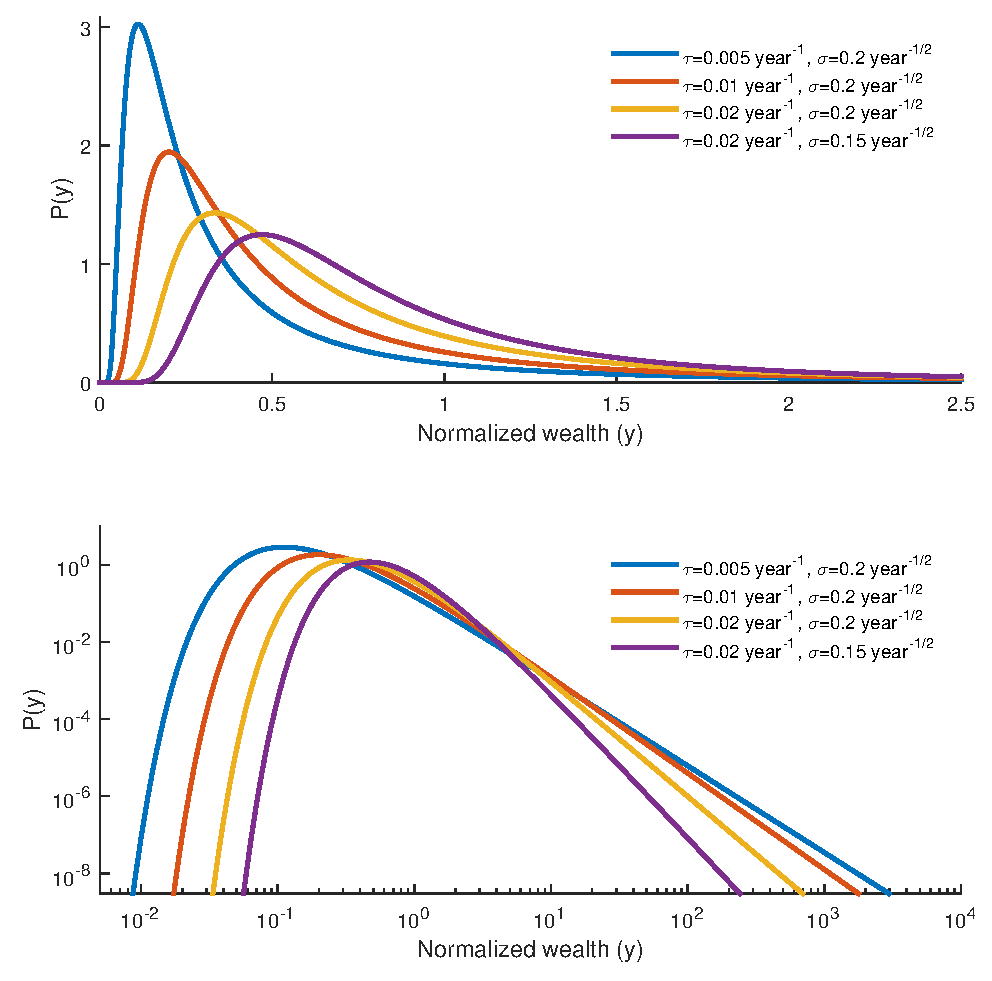
\includegraphics[width=1.0\textwidth] {./chapter_3/figs/dists.eps}
\caption{The stationary distribution for \RGBM with positive $\gphi$. Top -- linear scales; Bottom -- logarithmic scales.}
\flabel{dist}
\end{figure}

For positive reallocation, \eref{rgbm_ou_re} and extensions of it have received much attention in statistical mechanics and econophysics \cite{BouchaudMezard2000,Bouchaud2015}. As a combination of \GBM and a mean-reverting process it is a simple and analytically tractable stochastic process. \cite{LiuSerota2016} provide an overview of the literature and known results.

\paragraph{\underline{Negative $\gphi$}}
\mbox{}

For $\gphi<0$ the model exhibits mean repulsion rather than reversion. The ergodic hypothesis is invalid and no stationary wealth distribution exists. The population splits into those above the mean and those below the mean. Whereas in \RGBM with non-negative $\gphi$ it is impossible for wealth to become negative, negative $\gphi$ leads to negative wealth. No longer is total economic wealth a limit to the wealth of the richest individual because the poorest develop large negative wealth. The wealth of the rich in the population increases exponentially away from the mean, and the wealth of the poor becomes negative and exponentially large in magnitude, see \Fref{regimes}.

% AA comment on social mobility
Such splitting of the population is a common feature of non-ergodic processes. If rescaled wealth were an ergodic process, then individuals would, over long enough time, experience all parts of its distribution. People would spend 99 percent of their time as ``the 99 percent'' and 1 percent of their time as ``the 1 percent''. Therefore, the social mobility implicit in models that assume ergodicity might not exist in reality if that assumption is invalid. That inequality and immobility have been linked~\cite{Corak2013,LiuETAL2013,berman2017} may be unsurprising if both are viewed as consequences of non-ergodic wealth or income.

\begin{figure}[!htb]
\centering
\begin{tikzpicture}
%draw background
%\fill[draw=none, fill=lmlgrey, fill opacity=0.65] (0,0) rectangle (6,3);
%\fill[draw=none, fill=lmlgrey, fill opacity=0.25] (0,3) rectangle (6,6);

\fill[draw=none, pattern=north west lines, pattern color=black] (0,0.5) rectangle (5.9,3.5);
\fill[draw=none, pattern=crosshatch, pattern color=black] (0,3.5) rectangle (5.9,6.5);
\fill[draw=none, fill=white] (0.35,1) rectangle (5.55,3);
\fill[draw=none, fill=white] (0.35,4) rectangle (5.55,6);

%draw timeline
\draw [black,loosely dashed,ultra thick] (0,-0.5)--(0,0.5);
\draw[black,->,ultra thick,>=latex] (0,0.5)--(0,7.4) node[above left,rotate=90] {\small{ Reallocation rate ($\gphi$)}};
  
% draw ticks
\draw [black,ultra thick] (-0.2,3.5)--(0.0,3.5);	\draw (-0.2,3.5) 	node[left=3pt] {\normalsize{$\scriptstyle 0$}};

%draw regime lines


%draw text

\node[black,font={\normalsize},anchor=west,text width=5cm] at (0.375,2.0) {No stationary distribution exists; wealths diverge -- some positive, some negative};
\node[black,font={\normalsize},anchor=west,text width=5cm] at (0.375,5.0) {Stationary distribution exists; some moments converge, some don't};
%\node[black,font={\footnotesize},anchor=west] at (0.1,1.3) {- No stationary distribution;};
%\node[black,font={\footnotesize},anchor=west] at (0.1,1.0) {- };
%\node[black,font={\footnotesize},anchor=west] at (0.1,0.7) {\,\, some negative};
%\node[black,font={\footnotesize},anchor=west] at (0.1,3.3) {- Stationary distribution exists;};
%\node[black,font={\footnotesize},anchor=west] at (0.1,3) {- Some moments converge,};
%\node[black,font={\footnotesize},anchor=west] at (0.1,2.7) {\,\, some don't};

%embed figs
\node[anchor=west] at (6,3.4)  {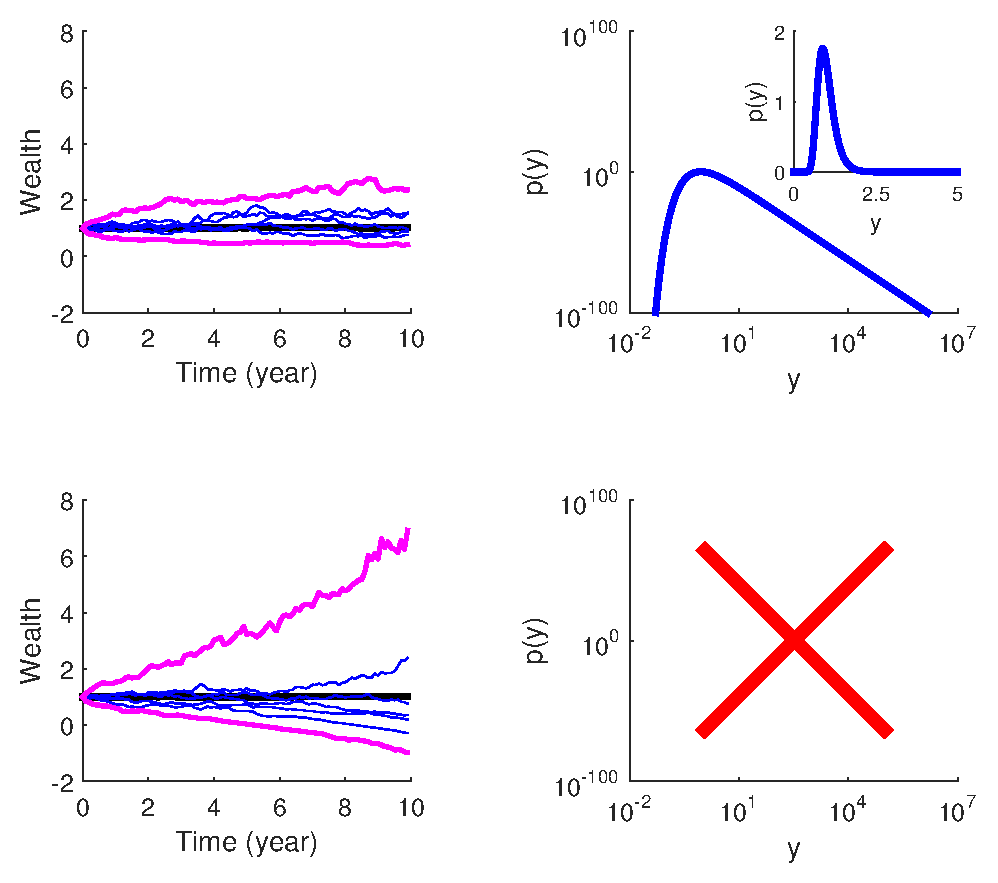
\includegraphics[height=6.5cm,keepaspectratio]{./chapter_3/figs/trajectories.eps}};
%\node[anchor=west] at (6,4.5)  {\includegraphics[height=3cm,keepaspectratio]{pos_tau1.eps}};
%\node[anchor=west] at (9.75,4.5)  {\includegraphics[height=3cm,keepaspectratio]{pos_tau3.eps}};
%\node[anchor=west] at (6,1.5)  {\includegraphics[height=3cm,keepaspectratio]{pos_tau2.eps}};

\draw [black,densely dashed,ultra thick] 			(0,3.5)--(13.5,3.5);

%labels
\node[black,font=\normalsize\sffamily,anchor=west,text width=4.5cm] at (0.2,6.75) {A)};
\node[black,font=\normalsize\sffamily,anchor=west,text width=4.5cm] at (5.85,6.75) {B)};
\node[black,font=\normalsize\sffamily,anchor=west,text width=4.5cm] at (9.7,6.75) {C)};
\node[black,font=\normalsize\sffamily,anchor=west,text width=4.5cm] at (5.85,3.15) {D)};
\node[black,font=\normalsize\sffamily,anchor=west,text width=4.5cm] at (9.7,3.15) {E)};
  
\end{tikzpicture}
\caption{Regimes of \RGBM. A) $\gphi=0$ separates the two regimes of \RGBM. For $\gphi>0$, a stationary wealth distribution exists. For $\gphi<0$, no stationary wealth distribution exists and wealths diverge. B) Simulations of \RGBM with $\N=1000$, $\gmu=0.021 \text{ year}^{-1}$ (presented after rescaling by $\exp(\gmu \t)$), $\gsigma=0.14\text{ year}^{-1/2}$, $\x_\gi\left(0\right)=1$, $\gphi=0.15 \text{ year}^{-1}$. Magenta lines: largest and smallest wealths, blue lines: five randomly chosen wealth trajectories, black line: sample mean. C) The stationary distribution to which the system in B) converges. Inset: same distribution on linear scales. D) Similar to B), with $\gphi=-0.15 \text{ year}^{-1}$. E) in the $\gphi<0$ regime, no stationary wealth distribution exists.}
\flabel{regimes}
\end{figure}

%%%%%%%%%%%%%%%%%%%%%%%%%%%%%%%%%%%%%%%

\subsubsection{Derivation of the stable distribution}
\seclabel{RGBM_stable}
In this section we will sketch the argument for why we can make the self-averaging approximation, \eref{rgbm_self}, in \RGBM with sufficiently fast positive reallocation, \eref{tau_c}. This is shown rigorously in \cite{Bouchaud2015b}. Then we will solve the Fokker-Planck equation for the rescaled wealth and derive the inverse gamma distribution, \eref{disti}.

We presented arguments in \secref{sketch} for why wealth in \GBM is self-averaging, $\ave{\x(\t)}_\N\sim\ave{\x(\t)}=\exp(\gmu \t)$ for short time. By mapping from \GBM to the random energy model in \secref{REM}, we showed that ``short time'' means $\t<t_c$, where $t_c=2\ln \N/\gsigma^2$. We can think of this as follows: $t_c$ is the timescale over which the inequality-increasing effects of noisy multiplicative growth drive wealths apart, such that a finite sample of wealths stops self-averaging and becomes dominated by a few trajectories.

Let's now think about what happens when we add reallocation to \GBM, creating \RGBM. $\gphi$ is the reallocation rate, so $\gphi^{-1}$ is reallocation timescale, \ie the timescale over which the inequality-reducing effects of reallocation pull wealths together. If $\gphi^{-1}>t_c$, then reallocation happens too slowly to prevent the expiry of self-averaging. However, if $\gphi^{-1}<t_c$, then reallocation pulls wealths together more quickly than they get driven apart, continually ``resetting'' the sample and allowing self-averaging to be maintained indefinitely. Converting this condition into a reallocation rate, we get $\gphi>{t_c}^{-1}$, as in \eref{tau_c}. As mentioned in \secref{RGBM_behaviour}, this becomes indistinguishable from $\gphi>0$ for realistic parameters, so the self-averaging approximation can be made safely for all positive $\gphi$ when using the model to study real economies.

We can now approximate the rescaled wealth, $y_\gi(\t)=\x_\gi(\t)/\ave{\x(\t)}_\N$, as $y_\gi(\t)=\x_\gi(\t)\exp(-\gmu \t)$. Using \Ito's formula as we did \secref{rescaled} yields the following SDE for rescaled wealth, now under \RGBM instead of \GBM:
\be
dy= \gsigma\,y\,\gd\gW - \gphi\left(y - 1\right)dt.
\ee
This is an It\^o equation with drift term $A=\gphi(y - 1)$ and diffusion term $B=y \gsigma$. Such equations imply ordinary second-order differential equations that describe the evolution of the \PDFa, called Fokker-Planck equations. The Fokker-Planck equation describes the change in probability density, at any point in (rescaled wealth) space, due to the action of the drift term (like advection in a fluid) and due to the diffusion term (like heat spreading). In this case, we have
\be
\frac{d\PDF\left(y,\t\right)}{dt}=\frac{\partial}{\partial y} \left[A\PDF\left(y,\t\right)\right]+\frac{1}{2} \frac{\partial^2}{\partial y^2}\left[B^2 \PDF\left(y,\t\right)\right].
\ee

The steady-state Fokker-Planck equation for the \PDFa, $\PDF\left(y\right)$, is obtained by setting the time derivative to zero,
\be
\frac{\gsigma^2}{2}\left(y^2 \PDF\right)_{yy} + \gphi\left[\left(y-1\right)\PDF\right]_y = 0.
\elabel{fokker_planck}
\ee
Positive wealth subjected to continuous-time multiplicative dynamics with non-negative reallocation can never reach zero. Therefore, we solve \Eref{fokker_planck} with boundary condition $\PDF\left(0\right)=0$ to give
\be
\PDF\left(y\right) = C\left(\zeta\right) e^{-\frac{\zeta-1}{y}}y^{-\left(1+\zeta\right)}\,,
\ee
where 
\be
\zeta = 1+\frac{2\gphi}{\gsigma^2}
\ee
and
\be
C\left(\zeta\right) = \frac{\left(\zeta -1\right)^\zeta}{\Gamma \left(\zeta \right)}\,,
\ee
with the gamma function $\Gamma\left(\zeta\right) = \int_0^\infty \x^{\zeta-1} e^{-\x}\,\mathrm{d}\x$. The distribution has a power-law tail as $y\to\infty$, resembling Pareto's oft-confirmed observation that the frequency of large wealths tends to decay as a power-law \cite{Pareto1897}. The exponent of the power-law, $\zeta$, is called the Pareto parameter and is one measure of economic inequality.

%%%%%%%%%%%%%%%%%%%%%%%%%%%%%%%%%%%%%%%

\subsubsection{Moments and convergence times}
\seclabel{RGBM_moments}
The inverse gamma distribution, \eref{disti}, has a power-law tail. This means that, for positive reallocation, while some of the lower moments of the stable rescaled wealth distribution may exist, higher moments will not. Specifically, the $k^\text{th}$ moment diverges if $k>\zeta$. 

If we find parameters consistent with positive reallocation when we fit our model to data, we will be interested in whether certain statistics -- such as the variance -- exist. We will also want to know how long it takes the distribution to converge sufficiently to its stable form for them to be meaningful. Here we derive a condition for the convergence of the variance and calculate its convergence time, noting also the general procedure for other statistics.

The variance of $y$ is a combination of the first moment, $\ave{y}$ (the ensemble average), and the second moment, $\ave{y^2}$:
\be
V(y)=\ave{y^2}-\ave{y}^2
\ee
Thus we need to find $\ave{y}$ and $\ave{y^2}$ in order to determine the variance.

The first moment of the rescaled wealth is, by definition, $\ave{y}=1$. To find the dynamic of the second moment, we start with the SDE for the rescaled wealth,
\be
\gd y = \gsigma y\gd\gW - \gphi\left(y - 1\right)\gd\t,
\elabel{rescaledSDE}
\ee
and follow a now familiar procedure. We insert $f\left(y,\t\right)=y^2$ into \Ito's formula,
\be
\gd f = \frac{\partial f}{\partial \t} \gd\t + \frac{\partial f}{\partial y} \gd y + \frac{1}{2}\frac{\partial^2 f}{\partial y^2} \gd y^2
\ee
to obtain
\be
\gd \left(y^2\right) = 2y\gd y + \gd y^2.
\elabel{diff2}
\ee
We substitute \eref{diff2} for $\gd y$ to get terms at orders $\gd\gW$, $\gd\t$, $\gd\gW^2$, $\gd\t^2$, and $\gd\gW\gd\t$. The scaling of \BM allows us to replace $\gd\gW^2$ by $\gd\t$ and we ignore terms at $o\left(\gd\t\right)$. This yields
\bea
\gd \left(y^2\right) = 2\gsigma y^2\gd\gW - \left(2\gphi-\gsigma^2\right) y^2\gd\t + 2\gphi y\gd\t.
%+ \gphi^2\left(y - 1\right)^2\,dt^2 - \st{\gphi\left(y - 1\right)\,\gsigma y\,\gd\gW\,dt}
\eea
Taking expectations on both sides and noting that $\ave{y}=1$ gives us an ordinary differential equation for the second moment:
\be
\frac{\gd\ave{y^2}}{\gd\t} = -\left(2\gphi - \gsigma^2\right) \ave{y^2} + 2\gphi
\elabel{avediff2}
\ee
with solution
\be
\ave{y\left(\t\right)^2} = \frac{2\gphi}{2\gphi - \gsigma^2} + \left(\ave{y\left(0\right)^2} - \frac{2\gphi}{2\gphi - \gsigma^2}\right) e^{-\left(2\gphi - \gsigma^2\right)\t}.
\elabel{avediff3}
\ee

The variance $V\left(\t\right)=\ave{y\left(\t\right)^2}-1$ therefore follows
\be
V\left(\t\right) = V_{\infty}+\left(V_0 - V_{\infty}\right)e^{-\left(2\gphi - \gsigma^2\right)\t}\,,
\elabel{var1}
\ee
where $V_0$ is the initial variance and
\be
V_{\infty} = \frac{2\gphi}{2\gphi - \gsigma^2}\,.
\elabel{varinf}
\ee
$V$ converges in time to the asymptote, $V_{\infty}$, provided the exponential in \eref{var1} is decaying. 
This can be expressed as a condition on $\gphi$
\be
\gphi > \frac{\gsigma^2}{2},
\ee
which is the same as the condition we noted previously for the second moment to exist: $\zeta>k$ where $k=2$.

Clearly, for negative values of $\gphi$ the condition cannot be satisfied, and the variance (and inequality) of the wealth distribution will diverge. In the regime where the variance exists, $\gphi > \gsigma^2/2$, it also follows from \eref{var1} that the convergence time of the variance is $1/\left(2\gphi - \gsigma^2\right)$.

As $\gphi$ increases, increasingly high moments of the distribution converge to finite values. The above procedure for finding the second moment (and thereby the variance) can be applied to the $k^\text{th}$ moment, just by changing the second power $y^2$ to $y^k$. Therefore, any other cumulant can be found as a combination of the relevant moments. For instance, \cite{LiuSerota2016} also compute the third cumulant.

%%%%%%%%%%%%%%%%%%%%%%%%%%%%%%%%%%%%%%%

\subsubsection{Fitting United States wealth data}
\seclabel{RGBM_data}
We have introduced the \RGBM model and understood its basic properties. It is a simple model of an interacting population of noisy multiplicative growers. We expect it to be more realistic than \GBM ($\gphi=0$) because we know that in the real world people interact. In particular, large populations have over centuries developed public institutions and infrastructure, to which everyone contributes and from which everyone benefits. At first glance, therefore, we might expect to find that \RGBM with positive $\gphi$ to fit real wealth data better than \GBM or, indeed, \RGBM with negative $\gphi$.

Additionally, if this is true and if associated convergence times are shorter than the timescales of policy changes, it would indicate that the ergodic hypothesis is warranted and a helpful modelling assumption. If not, then the hypothesis would be unjustified and could be acting as a serious constraint on models of economic inequality, generating misleading analyses and recommendations.

In \cite{BermanPetersAdamou2017} we fit the \RGBM model to historical wealth data from the United States for the last hundred years. We won't include full technical description of this empirical analysis here. It would be too long and our main aim is to communicate the ideas we use to think about problems and build models. If you want to know more, please read the paper (and let us know what you think!) However, the results are interesting and, to us at least, a little shocking, so we include a brief summary.

The basic setup is to fix the values of $\gmu$, $\gsigma$, and $\N$ in our \RGBM model using data about, respectively, aggregate economic growth, stock market volatility, and population data; and then to find, by numerical simulation of \eref{rgbm}, the time series of $\gphi(\t)$ values which best reproduces historical wealth shares in the United States. The wealth share, $S_q(\t)$, is a type of inequality measure. It is defined as the proportion of total wealth owned by the richest fraction $q$ of the population. So, for example, $S_{0.1}=0.8$ means that the richest $10\%$ of the population own $80\%$ of the total wealth. Reproducing the historical wealth shares is one way of reproducing approximately the level of inequality in the wealth distribution, and the nice thing is that economists Emmanuel Saez and Gabriel Zucman have estimated around a century's worth of wealth shares for the United States \cite{SaezZucman2014}.

Fitting the model to these data will address two main questions:
\bi
\item Is the ergodic hypothesis valid for rescaled wealth in the United States? For it to be valid, fitted values of $\gphi\left(\t\right)$ must be robustly positive.
\item If $\gphi\left(\t\right)$ is robustly positive, is convergence of of the distribution to its stable form fast enough for the distribution to be used as a representative of the empirical wealth distribution?
\ei
Note that we have relaxed the model slightly. $\gphi$ is a fixed parameter in \eref{rgbm} but we allow it to vary with time in our empirical analysis.

\Fref{tau} (top) shows the results of fitting the \RGBM model to the wealth share data in \cite{SaezZucman2014}. There are large annual fluctuations in $\gphi_q\left(\t\right)$ (black line) but we are more interested in longer-term changes in reallocation driven by structural economic and political changes. To show these, we smooth the data by taking a central 10-year moving average, $\widetilde{\gphi}_q\left(\t\right)$ (red line), where the window is truncated at the ends of the time series. We also show the uncertainty in this moving average (red envelope).

\begin{figure}[!htb]
\centering
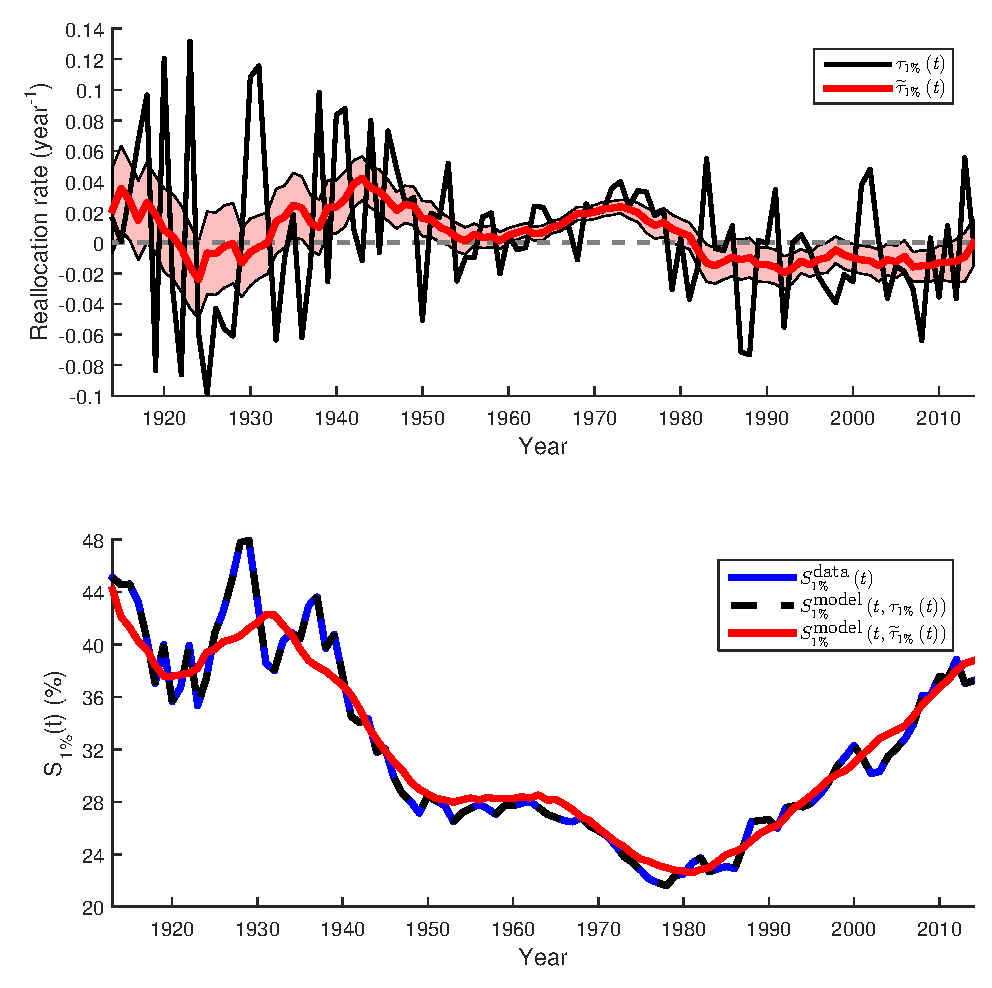
\includegraphics[width=1.0\textwidth] {./chapter_3/figs/tau_top1.eps}
\caption{Fitted effective reallocation rates. Calculations done using $\gmu=0.021 \text{ year}^{-1}$ and $\gsigma=0.16 \text{ year}^{-1/2}$. Top: $\gphi_{1\%}\left(\t\right)$ (black) and $\widetilde{\gphi}_{1\%}\left(\t\right)$ (red). Translucent envelopes indicate one standard error in the moving averages. Bottom: $S^{\text{data}}_{1\%}$ (blue), $S^{\text{model}}_{1\%}$ based on the annual $\gphi_{1\%}\left(\t\right)$ (dashed black), based on the 10-year moving average $\widetilde{\gphi}_{1\%}\left(\t\right)$ (red).}
\flabel{tau}
\end{figure}

To ensure the smoothing does not introduce artificial biases, we reverse the procedure and use $\widetilde{\gphi}_q\left(\t\right)$ to propagate the initially inverse gamma-distributed wealths and determine the wealth shares $S^{\text{model}}_q\left(\t\right)$. The good agreement with $S^{\text{data}}_q\left(\t\right)$ suggests that the smoothed $\widetilde{\gphi}_q\left(\t\right)$ is meaningful, see \Fref{tau} (bottom).

The ``take home'' is this: while the effective reallocation rate, $\widetilde{\gphi}\left(\t\right)$, was positive for most of the last hundred years, it was negative -- \ie reallocation from poorer to richer -- from the mid-1980s onwards. Furthermore, even when $\gphi\left(\t\right)$ was positive, associated convergence times (estimated both by numerical simulation and by plugging fitted model parameters into the results of \secref{RGBM_moments}) were very long compared to the typical times between policy changes -- from several decades to several centuries. This makes the answer to both our questions above a resounding ``No.''

What shocked us most when we first encountered these results was the existence of long periods with negative reallocation. We began the analysis imagining that \GBM (\ie $\gphi=0$, no interactions) was a really crazy model of the real world. After all, we personally pay our taxes and use public services, and the London Mathematical Laboratory is supported by generous charitable reallocations! We imagined that we would see $\gphi>0$ but that it might be so small that convergence times would be too long for the ergodic hypothesis to be useful. Instead we found that, recently in the Unites States at least, reallocation has been consistently negative. In our model, this corresponds to wealths being driven apart, populations splitting into groups with positive and negative wealths, and no convergence to a stable distribution of rescaled wealth.

In retrospect, perhaps we shouldn't have been so surprised. Qualitatively, our results echo the findings that the rich are experiencing higher growth rates of their wealth than the poor~\cite{Piketty2014,wolff2014household} and that the cumulative wealth of the poorest 50 percent of the American population was negative during 2008--2013~\cite{Rios20162013,WID2017}.

The economic phenomena that trouble theorists most -- such as diverging inequality, social immobility, and the emergence of negative wealth -- are difficult to reproduce in models that make the ergodic hypothesis. In our simple model, this is easy to see: in the ergodic regime, $\gphi>0$, our model cannot reproduce these phenomena at all. One may be tempted to conclude that their existence is a sign of special conditions prevailing in the real world -- collusion and conspiracies. But if we admit the possibility of non-ergodicity, $\gphi\leq0$, it becomes clear that these phenomena can easily emerge in an economy that does not actively guard against them.